% Build with custom engines, which move all miscellaneous files into a 'build' folder.
% See https://tex.stackexchange.com/questions/67211/use-texshop-preview-window-when-different-output-dir-is-set

%% ------ Packages ------ %%
% Related to the document setup:
\documentclass[12pt, a4paper]{extarticle}
\usepackage[a4paper, top = 2.4cm, bottom = 2.4 cm, right= 2.1cm, left= 2.1cm]{geometry}
\usepackage[english]{babel}
\renewcommand\familydefault{\sfdefault}
\usepackage{lmodern}
\usepackage{amsmath}
\usepackage{mathtools}
\usepackage{amsfonts}
\usepackage{amssymb}

\usepackage[T1]{fontenc}
\setlength\parindent{0pt}
\usepackage{multicol}
\usepackage{xspace}

\usepackage{tocloft}

% Colouring the references
\usepackage{hyperref}
\usepackage{cleveref}
\usepackage[dvipsnames]{xcolor}
\pagecolor{white}
\newcommand\myshade{85}
\colorlet{mylinkcolor}{violet}
\colorlet{mycitecolor}{YellowOrange}
\definecolor{myurlcolor}{rgb}{ 0, 0.4470, 0.6410}

\hypersetup{
  linkcolor  = mylinkcolor!\myshade!black,
  citecolor  = mycitecolor!\myshade!black,
  urlcolor   = myurlcolor!\myshade!black,
  colorlinks = true,
}

% Nomenclature
%\usepackage{nomencl}
%\makenomenclature
%%\renewcommand{\nomname}{List of symbols}
%\renewcommand{\nompreamble}{\noindent Definitions of the nomenclature}
%\newlength{\nomitemorigsep}
%\setlength{\nomitemorigsep}{\nomitemsep}
%\setlength{\nomitemsep}{-\itemsep}

% Section properties redefinitions
\makeatletter
\renewcommand\section{\@startsection {section}{1}{\z@}{3ex }{0.7ex } {\normalfont\large\bfseries}}
\renewcommand\subsection{\@startsection{subsection}{1}{\z@}{2ex }{0.1ex } {\normalfont \bfseries}}
\renewcommand\subsubsection{\@startsection{subsubsection}{3}{\z@}{-1.5ex\@plus -1ex \@minus -.2ex}{.5ex}{\normalfont}}
\makeatother

% Graphics interfaces:
\usepackage{graphicx}
\usepackage{tikz}
\tikzset{every picture/.style={line width=1pt}}
\usepackage{float}
\usepackage{subcaption} 
\usepackage[font=small,aboveskip=3pt, belowskip=-0pt]{caption}


% Headers and footers:
\usepackage{url}
\usepackage{footnote}
\usepackage{fancyhdr}
\pagestyle{fancy} 
\fancyhf{} 
\renewcommand{\headrulewidth}{0pt}
\newcommand{\mainmatter}{\clearpage \cfoot{\thepage\ of \pageref{LastPage}}
\setcounter{page}{1}
\pagenumbering{arabic}}
%\usepackage{comment}

\lfoot{\footnotesize \textcolor{Gray}{\thesistitle.}}
\rfoot{\footnotesize \textcolor{Gray}{\thesisauthor, \studentnumber. \thedate.}}
\fancyhfoffset{0pt}


% Sort the bibliography and add to the table of contents
\usepackage[sort]{cite}
\setlength\columnsep{15pt}
\usepackage[nottoc,numbib]{tocbibind}

% Redefine the \left and \right operators:
\let\originalleft\left
\let\originalright\right
\renewcommand{\left}{\mathopen{}\mathclose\bgroup\originalleft}
\renewcommand{\right}{\aftergroup\egroup\originalright}

% Redefine \eqref environment
\usepackage{letltxmacro}
\LetLtxMacro{\originaleqref}{\eqref}
\renewcommand{\eqref}{Equation~\originaleqref}

% Command definitions and macros:
\newcommand{\ic}{{\rm{i}}\xspace}
\renewcommand{\Re}{{\operatorname{Re}}\xspace}
\renewcommand{\Im}{{\operatorname{Im}}\xspace}

\newcommand{\Pulse}{{\mathcal{P}}\xspace}
\newcommand{\kmean}{{\langle k\rangle}\xspace}
\renewcommand{\k}{{\boldsymbol{k}}\xspace}
\newcommand{\kacc}{{\boldsymbol{k'}}\xspace}
\newcommand{\kin}{{k^{\rm in}}\xspace}
\newcommand{\kout}{{k^{\rm out}}\xspace}
\newcommand{\kinb}{{\boldsymbol{k^{\rm in}}}}
\newcommand{\koutb}{\boldsymbol{{k^{\rm out}}}}
\newcommand{\kinbi}{{\boldsymbol{k}_i^{\bf in}}}
\newcommand{\koutbj}{{\boldsymbol{k}_j^{\bf out}}}
\newcommand{\degree}{{\rm deg}\xspace}
\newcommand{\kmin}{k_{\text{min}}\xspace}
\newcommand{\kmax}{k_{\text{max}}\xspace}

\newcommand{\Sin}{{S^{\rm in}}\xspace}
\newcommand{\Sout}{{S^{\rm out}}\xspace}

\newcommand{\dtheta}{{\dot{\theta}}\xspace}

\newcommand{\permute}{{\digamma}\xspace}
\newcommand{\permuteinv}{{\digamma^{-1}}\xspace}

%\newcommand{\R}{{\rm I\!R}\xspace}
\newcommand{\R}{{\mathbb{R}}\xspace}
\renewcommand{\c}{{\mathbb{C}}\xspace}
\newcommand{\C}{\mathbb{C}_\circ}
\newcommand{\T}{{\mathbb{T}}\xspace}
\newcommand{\K}{{\mathbb{K}}\xspace}

\newcommand{\tp}{{t^{\prime}}\xspace}
\newcommand{\tpp}{{t^{\prime \prime}}\xspace}

\newcommand{\QIF}{{\textsl{QIF}}\xspace}
\newcommand{\PRC}{{\textsl{PRC}}\xspace}
\newcommand{\pdf}{{\textsl{pdf}}\xspace}
\newcommand{\MFR}{{\textsl{MFR}}\xspace}
\newcommand{\SNIC}{{\textsl{SNIC}}\xspace}
\newcommand{\PSR}{{\textsl{PSR}}\xspace}
\newcommand{\PSS}{{\textsl{PSS}}\xspace}
\newcommand{\CPW}{{\textsl{CPW}}\xspace}
\newcommand{\STDP}{{\textsl{STDP}}\xspace}
\newcommand{\ISI}{{\textsl{ISI}}\xspace}
\newcommand{\IP}{{\textsl{IP}}\xspace}



\def\matlab{\textsc{Matlab}\xspace}

% Author macros:
\newcommand{\thesistitle}{The dynamics of adaptive neuronal networks}
\newcommand{\thesissubtitle}{influence of topology on synchronisation }
\newcommand{\mywork}{{\textsl{Investigation:}}\xspace}

\newcommand{\thesisauthor}{Simon Aertssen} % Your name :) 
\newcommand{\studentnumber}{s181603}
\newcommand{\thedate}{February 1$^{\text{st}}$ 2021} 
\newcommand{\thesissupervisorI}{Erik Martens} 
\newcommand{\thesissupervisorII}{Poul Hjorth} 

\newcommand{\department}{DTU Compute}
\newcommand{\departmentdescriber}{Department of Applied Mathematics and Computer Science}
\newcommand{\addressI}{Richard Petersens Plads, Building 324}
\newcommand{\addressII}{2800 Kgs. Lyngby, DK}
\newcommand{\departmentwebsite}{www.compute.dtu.dk}


%% ------ Front page ------ %%

\begin{document}

\mainmatter

\pagenumbering{Roman}
% !TEX root = ../main.tex

\begin{titlepage} % Suppresses displaying the page number on the title page and the subsequent page counts as page 1
	\newcommand{\HRule}{\rule{\linewidth}{0.5mm}} % Defines a new command for horizontal lines, change thickness here
	
	%\center % Centre everything on the page
	
	%------------------------------------------------
	%	Headings
	%------------------------------------------------
	\begin{minipage}{\linewidth}
   	\begin{flushright}
	Msc thesis\\ Mathematical Modelling and Computation
    	\end{flushright}
 	\end{minipage}
	
	\begin{center} \begin{minipage}{0.87\linewidth}
	\begin{tikzpicture}[remember picture,overlay]
    		\node[anchor=south west,yshift=64pt,xshift=55pt]%
        		at (current page.south west)
        		{
\includegraphics[height=14mm]{../Figures/Logos/ComputeLogo.png}};
	\end{tikzpicture}
	\begin{tikzpicture}[remember picture,overlay]
    		\node[anchor=south east,yshift=64pt,xshift=-55pt]%
        		at (current page.south east)
        		{
\includegraphics[height=14mm]{../Figures/Logos/DTUlogoRed.png}};
	\end{tikzpicture}

	\end{minipage} \end{center}
	\vspace{100mm}
	
	
	%{\Large \department}\\[1.5cm] % Main heading such as the name of your university/college
	
	%{\large \departmentdescriber}\\[0.5cm] % Major heading such as course name
		
	%------------------------------------------------
	%	Title
	%------------------------------------------------
	
	%\HRule\\[0.4cm]
	
	{\Huge \thesistitle: \\ \thesissubtitle}\\% Title of your document
	
	%\HRule\\[1.5cm]
	
	%------------------------------------------------
	%	Author(s)
	%------------------------------------------------
	
	\begin{minipage}{0.5\textwidth}
		\begin{flushleft}
			\Large
			\thesisauthor, \studentnumber
		\end{flushleft}
	\end{minipage} \\[15mm]
	\begin{minipage}{\textwidth}
		\begin{flushleft}
			\large
			\textit{Supervisors}\\
			\thesissupervisorI \\
			\thesissupervisorII
		\end{flushleft}
	\end{minipage}
	
	% If you don't want a supervisor, uncomment the two lines below and comment the code above
	%{\large\textit{Author}}\\
	%John \textsc{Smith} % Your name
	
	%------------------------------------------------
	%	Date
	%------------------------------------------------
	
	\vfill % Position the date 3/4 down the remaining page
	
	{\large\thedate} % Date, change the \today to a set date if you want to be precise
	
	%------------------------------------------------
	%	Logo
	%------------------------------------------------
	
	%\vfill\vfill
	%\includegraphics[width=0.2\textwidth]{placeholder.jpg}\\[1cm] % Include a department/university logo - this will require the graphicx package
	 
	%----------------------------------------------------------------------------------------
	
	\vfill
	\begin{minipage}{\textwidth}
		\begin{flushleft}
			\small
			\department. \departmentdescriber. 
			\addressI, 	\addressII. \departmentwebsite	\\[0.2cm]
		\end{flushleft}
	\end{minipage}
	
	\vfill % Push the date up 1/4 of the remaining page

\end{titlepage}

\tableofcontents

\section*{Abstract}
\addcontentsline{toc}{subsection}{Abstract}
The synchronisation of networks of oscillators, network topology and network plasticity can only be understood using a holistic approach, and each domain is investigated in relation to the other. The Theta neuron model is analysed to understand feedback mechanisms between the electrical current and the phase response. Different network topologies are then described in terms of their degree distribution. Networks of Theta neurons are studied using the synchronisation of the mean-field. Inspired by the process of synaptic plasticity, learning rules are then established to observe emergent network topologies. 

%\section*{Acknowledgements}
%\addcontentsline{toc}{subsection}{Acknowledgements}
%thankyou thankyou thankyou thankyou thankyou thankyou thankyou thankyou thankyou thankyou thankyou thankyou thankyou thankyou thankyou thankyou thankyou thankyou thankyou thankyou thankyou thankyou thankyou thankyou thankyou thankyou thankyou thankyou thankyou thankyou thankyou thankyou thankyou thankyou thankyou thankyou thankyou thankyou thankyou thankyou thankyou thankyou thankyou thankyou thankyou thankyou thankyou thankyou 
%


% !TEX root = ../main.tex
\newpage
\section{Nomenclature}
\vspace{-.5cm}
\begin{alignat*}{2}
& \ic, e \text{ (or} \exp\text{)} &&\text{Imaginary unit. Euler's number.}\\ \\
& n, \degree(n) &&\text{Network node. Degree of node $n$.}\\
& N &&\text{Network degree. The number of neurons in the network.}\\
& A_{ij} &&\text{Adjacency matrix. Models which neuron $i$ is connected to neuron $j$ and vice-versa.}\\
& \kmean &&\text{Average node degree in the network.}\\
& \k &&\text{Node degree. Vector of the in- and out-degree of a single node as $\left(\kin, \kout \right)$.}\\
& \kinb, \koutb && \text{Node degree vector of all in- and out degrees of the network.} \\
& M_{\k} &&\text{Number of unique node degrees in the network.}\\
& P(k), P(\k) &&\text{Univariate and bivariate network degree distribution.}\\
&\kmin, \kmax &&\text{Smallest and largest degree found in a network.}\\ 
&\gamma &&\text{Degree exponent of a scale-free network.}\\ 
&p &&\text{Probability threshold of forming a link in random networks.}\\ 
&c &&\text{Assortativity of the network.}\\ \\
&\theta(t)_i &&\text{Phase variable function of the theta model (of neuron $i$).}\\
& \Pulse_n (\theta)&&\text{Pulse shaped synaptic coupling function.}\\
&\kappa &&\text{Macroscopic coupling strength.}\\
&\eta_i, I(t)_i &&\text{Excitability threshold and input current (of neuron $i$).}\\
&g(\eta \rvert \eta_0, \sigma) \quad &&\text{Excitability threshold distribution with mean $\eta_0$ and width $\sigma$.}\\ \\
& Z(t) &&\text{Kuramoto order parameter function.}\\
& z(\k, t) &&\text{Order parameter function for nodes with degree $\k$.}\\
& \bar{Z}(t) &&\text{Mean field order parameter function for arbitrary networks.}\\ \\
& \Sin(t)_i, \Sout(t)_i \quad &&\text{Spike trains received and emitted by neuron $i$ as a sum of delta functions in time.}\\ 
& K_{ij} &&\text{Synaptic connectivity matrix. Strength of the connections between neurons $i$ and $j$.}\\
& \Delta t_{ij} &&\text{Time difference between spikes of neurons $i$ and $j$.}\\
& W(\Delta t_{ij}) &&\text{Learning window. Models the correlation between synaptic strength and spike times.}\\ 
& \phi(\Delta t_{ij}) &&\text{IP learning function. Models correlation between excitability strength and spike times.}\\ \\
& \T &&\text{Set of angles in [-$\pi$, $\pi$[.}\\
& \K &&\text{Set of unique degrees in a network, support of $P$.}\\ 
& \R, \C &&\text{Set of real numbers. Set of complex numbers.}\\ \\
& \permute(v), \permuteinv(v) &&\text{Random permutation and inverse permutation of the elements of a vector $v$.}\\ 
\end{alignat*}

% !TEX root = ../main.tex
\newpage
\section{Introduction}
\noindent In 2013, one of the largest scientific projects ever funded by the European Union was launched. With the Human Brain Project \cite{humanbrainproject}, scientists and researchers aimed to reconstruct the human brain through supercomputer-based models and to advance neuroscience, medicine, and computing. Across the globe different fields of science are drawing inspiration from the human brain, through different approaches. \\
One such approach is to model the behaviour of biological neurons and to quantify the information processes in the brain from stimuli from the senses or from electrical and chemical processes in the body. A given neuron receives hundreds of impulses in the form of neurotransmitters, almost exclusively on its dendrites and cell body. These stimuli add up to an excitatory or inhibitory influence on the membrane potential of the neuron, so that the potential spikes when excitation is higher than an internal threshold. At this point, the neuron releases its own neurotransmitter and joins the interneuronal communication \cite{IntroductionModelingDynamics}. The neuron dynamics are largely captured by this spiking behaviour, on which most efforts have been concentrated.
In 1952, Hodgkin and Huxley described a mathematical model for the action potentials in neurons, using a set of nonlinear differential equations that approximates the electrical characteristics of the neuron elements. In 1963 the authors were awarded the Nobel Prize in Physiology or Medicine \cite{nobel1963} for their work.\\
As the human brain contains more than 100 billion neurons \cite{Herculano2009} it is unfeasible to study complex models at this scale. The topology of neuronal networks displays traits of small-worldness, wiring optimisation, and heterogeneous degree distributions \cite{Bullmore2010}, for which it is difficult to pin down one type of network architecture. Through the mean-field reduction (\MFR) proposed in \cite{OttAntonsen2008} one can reduce a large network of indistinguishable neurons to a low-dimensional dynamical system, described by the attraction of a mean-field variable to a reduced manifold.
In this paper we will study the \MFR of different types of networks of coupled theta neurons using the generalisations found in \cite{OttAntonsen2017}.

We distinguish between two types of dynamics: we study the dynamics of pulse-coupled networks \textsl{on} networks, and the dynamics \textsl{of} such networks is how they evolve over time. The dynamics of the network occur on a different (slower) time-scale than the dynamics on the network. Both types of dynamics influence each other \cite{AdaptiveNetworks2009}.

\renewcommand{\thepage}{\arabic{page}}

% !TEX root = ../main.tex
\newpage
\section{\theory The Theta Neuron Model} \label{TheThetaNeuronModel}
%\subsection{Canonical neuron models}
A number of neuron model families have been identified, and often there exists a continuous change of variables from models of the same family into a \textit{canonical} model that can represent the whole family \cite{Hoppensteadt2001CanonicalNM}. As the transformation is not required to be invertible, we can study the universal neurocomputational properties of the family in a low dimensional model.
It was Hodgkin \cite{Hodgkin1948} who classified neurons into two types based on their excitability, upon experimenting with the electrical stimulation of cells. Class 1 models begin to spike at an arbitrarily slow rate, and the spiking frequency increases when the applied current is increased. Class 2 models spike as soon as their internal threshold is exceeded and the spiking frequency stays relatively constant within a certain frequency band \cite{Hoppensteadt2001CanonicalNM}.


\subsection{Theta Neuron model description} \label{sec:TheThetaNeuronModelDescription}
In \cite{Ermentrout1986}, a Class 1 canonical phase model was proposed:
\begin{align}
\dot{\theta} = (1-\cos \theta)+(1+\cos \theta) \cdot I \qquad \theta \in \T \label{eq:thetaneuron}
\end{align}
with $I$ a bifurcation parameter on the supplied current. We can visualise the dynamics on the unit circle, like in Figure \ref{fig:thetaneuronbifurcationtikz}. The neuron produces a spike when $\theta$ surpasses $\pi$, upon which $\theta \leftarrow -\pi$. 

\begin{figure}[H]
\minipage{0.33\linewidth}
\centering
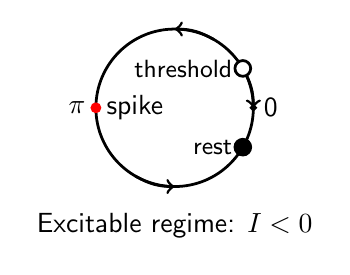
\begin{tikzpicture}
    \draw (0,0) circle [radius=1];
    \draw (0,-1.2) node[below]{Excitable regime: $I < 0$};
    \draw (-1,0) node[left]{$\pi$};
    \draw[fill=black, black] (1,0) circle [radius=0.025];
    \draw (1,0) node[right]{0};
    \draw[fill=red, red] (-1,0) circle [radius=0.05];
    \draw (-1,0) node[right]{spike};
    
    \draw[black, ->] (0.866, 0.5)to[out=-60,in=90](1,0);
    \draw[fill=white, draw=black] (0.866,0.5) circle [radius=0.1];
    \draw (0.866,0.5) node[left]{\small{threshold}};
    
    \draw[fill=black, draw=black] (0.866,-0.5) circle [radius=0.1];
    \draw (0.866,-0.5) node[left]{\small{rest}};
    
    \draw[black, ->] (0.5,0.866)to[out=150,in=0](0,1);
    \draw[black, ->] (-0.5,-0.866)to[out=-30,in=180](0,-1);
\end{tikzpicture}
\endminipage
\minipage{0.33\linewidth}
\centering
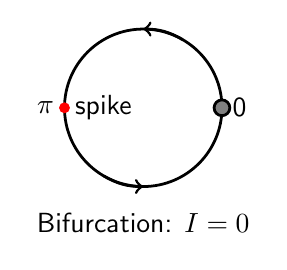
\begin{tikzpicture}
    \draw (0,0) circle [radius=1];
    \draw (0,-1.2) node[below]{Bifurcation: $I = 0$};
    \draw (1,0) node[right]{0};
    \draw[fill=red, red] (-1,0) circle [radius=0.05];
    \draw (-1,0) node[right]{spike};
    \draw (-1,0) node[left]{$\pi$};
    
    \draw[fill=gray, draw=black] (1,0) circle [radius=0.1];
    
    \draw[black, ->] (0.5,0.866)to[out=150,in=0](0,1);
    \draw[black, ->] (-0.5,-0.866)to[out=-30,in=180](0,-1);
\end{tikzpicture}
\endminipage
\minipage{0.33\linewidth}
\centering
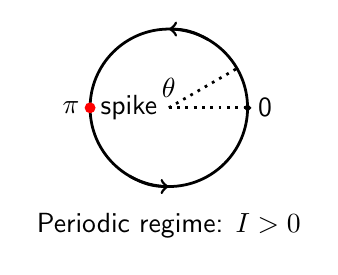
\begin{tikzpicture}
    \draw (0,0) circle [radius=1];
    \draw (0,-1.2) node[below]{Periodic regime: $I > 0$};
    \draw (-1,0) node[left]{$\pi$};
    \draw (1,0) node[right]{0};
    \draw[fill=black, black] (1,0) circle [radius=0.025];
    \draw[fill=red, red] (-1,0) circle [radius=0.05];
    \draw (-1,0) node[right]{spike};
    
    \draw[black, dotted] (0,0)to(1,0);
    \draw(0,0) node[above]{$\theta$};
    \draw[black, dotted] (0,0)to(0.866,0.5);
    
    \draw[black, ->] (0.5,0.866)to[out=150,in=0](0,1);
    \draw[black, ->] (-0.5,-0.866)to[out=-30,in=180](0,-1);
\end{tikzpicture}
\endminipage
\caption{SNIC bifurcation of the theta neuron model. A spike occurs when $\theta = \pi$. For $I < 0$, the neuron is in a rest state but \textsl{excitable} and we observe one stable and one unstable equilibrium point. For $I > 0$, $\dot{\theta} > 0$ so that $\theta$ moves continuously around the circle and we can observe \textsl{periodic} sustained spiking. The saddle-node bifurcation occurs at $I = 0$, so that $\theta$ will spike when it is larger than 0.}
\label{fig:thetaneuronbifurcationtikz}
\end{figure}

We can recognise the features of the class 1 model in Figure \ref{fig:ThetaNeuronResponseToCurrent}. This makes \eqref{eq:thetaneuron} the normal form of the \textit{saddle-node-on-invariant-circle} ($\SNIC$) bifurcation \cite{Luke2013}, as it collapses $\R$ to $\T$.

\begin{figure}[H]
\centering
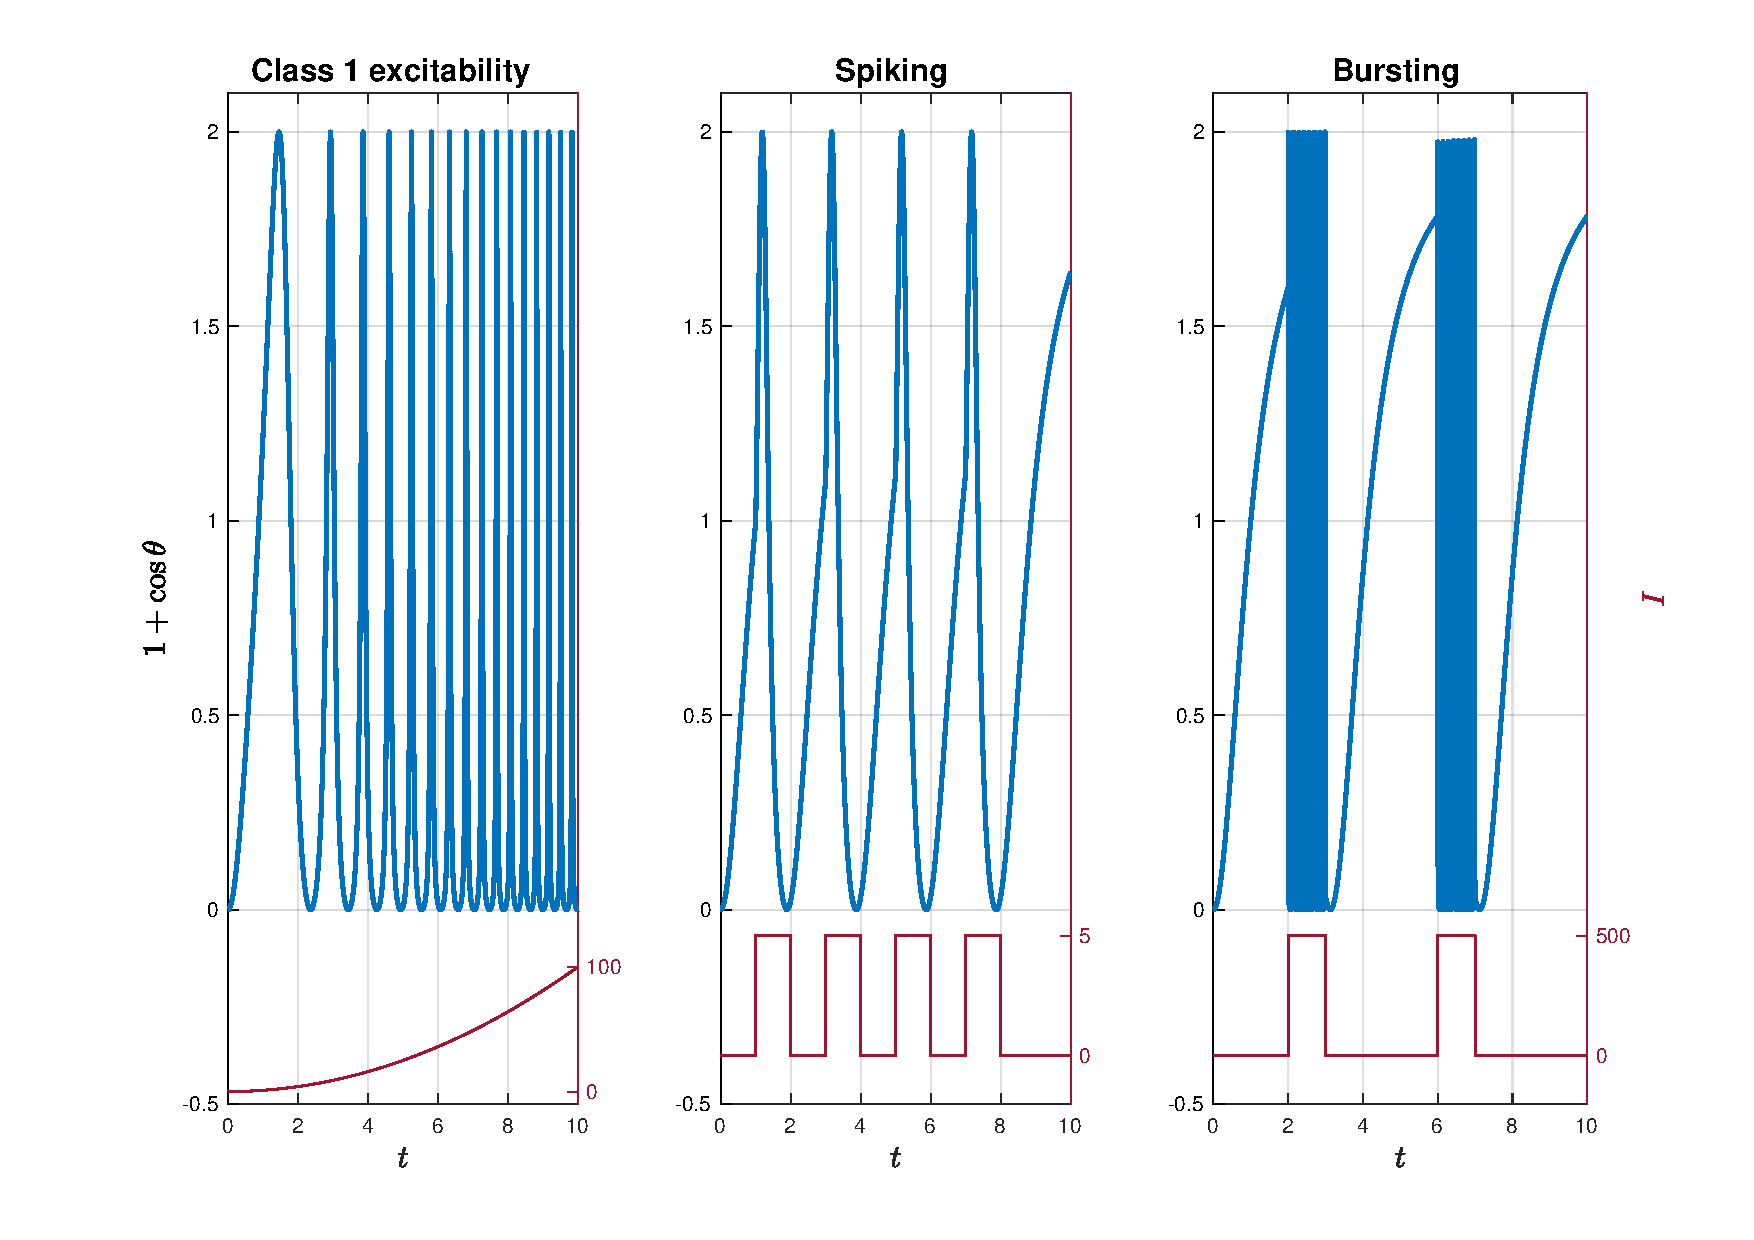
\includegraphics[width = \textwidth]{../Figures/ThetaNeuronResponseToCurrent.pdf}
\caption{Properties of the theta neuron model, with solutions of \eqref{eq:thetaneuron} in blue, spikes marked in dotted lines, and the current $I$ in red. Left: the spike frequency of $\theta$ increases as $I$ is increased over time, which is the distinguishing feature of class 1 canonical models. Middle: spikes occur within a finite time period when $I > 0$ and within infite time when $I = 0$. Right: when $I$ is large, the neuron \textsl{bursts}.}
\label{fig:ThetaNeuronResponseToCurrent}
\end{figure}

Equilibria only exist for the \textsl{excitable} regime $I < 0$: 
\begin{align*}
\dot{\theta} &= 1-\cos \theta+I+I \cdot \cos \theta = (I+1)+(I-1) \cdot \cos \theta \\
\theta^{\ast}_{1, 2} &= \pm \arccos \left(\frac{I+1}{1-I}\right)+2 \pi n
\end{align*}
We can find the stability of the equilibria through:
\begin{align*}
\frac{\mathop{d}}{\mathop{d \theta}}((1-\cos \theta)+(1+\cos \theta) \cdot I) &= \sin \theta-\sin \theta \cdot I = (1-I) \cdot \sin \theta
\end{align*}
In the equilibria this yields:
\begin{align*}
\frac{\mathop{d}}{\mathop{d \theta}}\left( \theta^{\ast}_{1, 2} \right) &= \pm(1-I) \cdot \sqrt{1 - \left( \frac{I+1}{1-I} \right)^2 } = \pm(1-I) \cdot \frac{2 \sqrt{-I}}{1-I} = \pm2 \sqrt{-I}
\end{align*}
We find that $\theta^{\ast}_{1}$ is an unstable equilibrium point, and that $\theta^{\ast}_{2}$ is stable. This means that as $\theta$ gets perturbed above $\theta^{\ast}_{1}$, a spike occurs and $\theta$ converges to $\theta^{\ast}_{2}$. This is demonstrated in Figure \ref{fig:ThetaModelEquilibriumPoints}.
\begin{figure}[H]
\centering
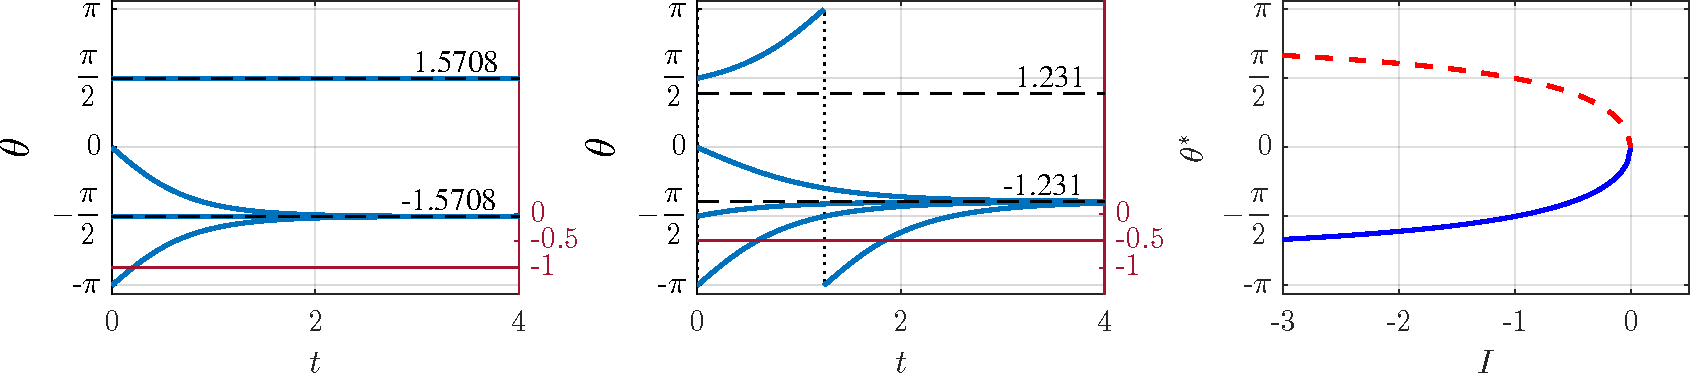
\includegraphics[width = \textwidth]{../Figures/ThetaModelEquilibriumPoints.pdf}
\caption{Equilibria $\theta^{\ast}$ for different values of $I < 0$. Left: $I = -1$ yields $\theta^{\ast}_{1,2} = \pm \frac{\pi}{2}$, one of the simulations is started exactly on the unstable equilibrium and stays there. Middle: $I = -0.5$, we see how a spike occurs when $\theta > \theta^{\ast}_{1}$ upon which $\theta \rightarrow \theta^{\ast}_{2}$. Right: bifurcation diagram of the \SNIC bifurcation, with the stable equilibria in blue, and the unstable in red. At $I = 0$ the equilibria merge into one.}
\label{fig:ThetaModelEquilibriumPoints}
\end{figure}


\subsection{Solutions for static currents} \label{sec:TheThetaNeuronModelSolutionPeriodics}
Gaining insight into \eqref{eq:thetaneuron} is hard, due to the difficulty of finding an analytical solution. However, it has been noted that there exists a simple transformation which yields (see \ref{app:TransformationToQIF}):
\begin{align}
V &\equiv \tan \left( \frac{\theta}{2} \right) \label{eq:QIFtransformation} \\
\dot{V} &= V^2 + I \label{eq:QIFmodel}
\end{align}
This model is called the \textsl{Quadratic Integrate and Fire model} (\QIF). \eqref{eq:QIFmodel} models the membrane potential of a neuron, which spikes at $V=\infty$ and resets to $V \leftarrow -\infty$. The transformation \eqref{eq:QIFtransformation} is continuous between spikes, so insights from a solution for $V$ can be transformed directly to $\theta$. The equilibria of the \QIF model are simply $\pm \sqrt{-I}$ (as $I < 0$) so that we can express $\theta^{\ast}_{1, 2} = 2 \arctan \left( \pm \sqrt{-I} \right)$ \cite{Gutkin2014}. \\

The solution for the excitable regime $I < 0$ is :
\begin{align}
V(t) = \frac{2 \sqrt{-I}}{1 - e^{2 t \sqrt{-I}}}-\sqrt{-I} \label{eq:ThetaNeuronModelSolutionPeriodicExcitable}
\end{align}
The solution at the bifurcation $I = 0$ is :
\begin{align}
V(t) = \frac{-1}{t} \label{eq:ThetaNeuronModelSolutionPeriodicBifurcation}
\end{align}
The solution for the periodic regime $I > 0$ is :
\begin{align}
V(t) = -\sqrt{I} \cdot \cot (t \sqrt{I}) \label{eq:ThetaNeuronModelSolutionPeriodic}
\end{align}
These equations assume that at $t=0$ a spike has occured. The steps required to find the solutions (\ref{eq:ThetaNeuronModelSolutionPeriodicExcitable}) to (\ref{eq:ThetaNeuronModelSolutionPeriodic}) are described in \ref{app:ThetaModelSolutions}. Solutions for $\theta$ are found by simply taking the inverse of the transformation in \eqref{eq:QIFtransformation}.

If the \QIF model is so much simpler, then why bother using the Theta model? Simulating the \QIF model requires an artificial reset threshold, because we cannot expect a computer to represent infinity easily. Finite thresholds make the analytical solutions more difficult and convoluted. By using the Theta model the dynamics remain smooth and bounded on $\T$. %Since we take the cosine of the phase angle in \eqref{eq:thetaneuron}, we do not even


\subsection{Numerical solutions} \label{sec:TheThetaNeuronModelODE45}
When $I$ is not static, we need to revert to numerical solutions. A fixed-step 4-stage Runge-Kutta method (Dormand-Prince 45) was implemented to numerically solve all differential equations. A fixed-step algorithm makes it possible to finely tune the large memory demand of the systems presented in this work. 


\subsection{Frequency response} \label{sec:TheThetaNeuronModelFrequencyResponse}
\setlength\intextsep{0pt}
\begin{wrapfigure}{r}{0.39\textwidth}
\centering
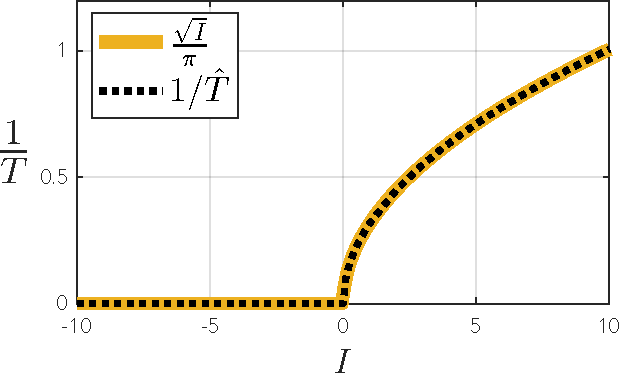
\includegraphics[width = \linewidth]{../Figures/ThetaNeuronfI.pdf}
\caption{Frequency response of the Theta model. For $I \leq 0$ the spike period is infinite, which is why we see the solutions to (\ref{eq:thetaneuron}) approach $\theta = 0$ for $I = 0$ in Figure \ref{fig:ThetaNeuronResponseToCurrent}. }
\label{fig:ThetaNeuronfI}
\end{wrapfigure}
As we already saw in Figure \ref{fig:ThetaNeuronResponseToCurrent}, an increasing current increases the spiking frequency. We can compute this relationship by measuring how long it takes for $V$ to reach a spike: we solve \eqref{eq:ThetaNeuronModelSolutionPeriodic} for $t$ at $V(t) = +\infty$ in \ref{app:ThetaModelFrequencyResponse}. This yields the oscillation period $T = \frac{\pi}{\sqrt{I}}$, which we can see in Figure \ref{fig:ThetaNeuronfI}. 

We know that when $\theta > \theta^{\ast}_{1}$ a spike occurs in the excitable regime, or in any case in the periodic regime. But the time that it takes to reach the spike can be arbitrarily long, depending on how far we are over $\theta^{\ast}_{1}$. So, spikes will occur, but after a delay that is dependant on the stimulus. Explicitly, if we perturb $\theta(0) = \theta^{\ast}_{1} + \varepsilon$ we obtain from \cite{Gutkin2014}:
\begin{align*}
T_{\text {spike}} = \frac{-\tanh ^{-1}\left(1+\frac{\epsilon}{\sqrt{I}}\right)}{\sqrt{I}}
\end{align*}
The delay to the spike blows up as $\varepsilon \rightarrow$ 0 so that spikes may occur after a very large delay. \\

In most of our future work, $I$ will not be a static current. We ask ourselves: how sensitively does $T$ depend on $I$ when $I$ is perturbed? We can measure this as a \textsl{relative} perturbation using $\mathop{dI}/I$ and $\mathop{dT/T}$ \cite{IntroductionModelingDynamics} :
\begin{align*}
\left| \frac{dT}{dI} \frac{I}{T} \right| &= \left| \frac{dT / T}{dI / I}\right| 
= \left|- \frac{\pi}{2} \left(\frac{1}{\sqrt{I}}\right)^3 \frac{I}{T} \right| 
= \left| \frac{\pi}{2} \left(\frac{T}{\pi}\right)^3 \frac{I}{T} \right| 
= \frac{1}{2} \left|\left(\frac{T}{\pi}\right)^2 \left(\frac{\pi}{T}\right)^2 \right| = \frac{1}{2}
\end{align*}
Hence, a 1\% change in $I$ will result in a 0.5 \% change in the period.


\subsection{Phase response} \label{sec:TheThetaNeuronModelPhaseResponse}
Perturbations on the period can also be understood from the perspective of the phase. Changes to the phase $\theta$ can delay or advance the event of a spike, and in general this depends on exactly when the stimulus occurs. The phase response curve (\PRC) gives us exactly that relation \cite{Perez2020, Gutkin2014}.

Let us define $\phi \in [0, T[$, which represents the time since the last event of a spike. When we add a small bifurcation $\varepsilon$ to $\theta$ at time $\phi$, a spike will occur at $T_{\phi}$, and we have that $\theta(\phi_{\rm new}) = \theta(\phi) + \varepsilon$. The time to the new spike is $T_{\phi} = T + (\phi - \phi_{\text{new}})$. The \PRC can then be defined as:
\begin{align}
\PRC(\phi) =T_{\phi} - T \label{eq:PRC1}
\end{align}
The \PRC is thus the expected delay of the the phase period in function of the timing of the delay. This process has been visualised in Figure \ref{fig:ThetaNeuronfIPRC}, after \cite{Perez2020}. For infinitesimally small perturbations to the phase, we can find the \PRC as the \textsl{adjoint} of the solution \cite{Gutkin2014}:
\begin{align}
\PRC(\phi) = \frac{1}{d V(\phi) / d \phi} = \frac{1}{2 \sqrt{I}} \left(1-\cos \left( \frac{2 \pi}{T} \phi \right) \right) \label{eq:PRC2}
\end{align}
We can use $\phi \in [0, T[$ and $\theta \in \T$ to see that \eqref{eq:PRC2} can be expressed as:
\begin{align}
\PRC(\theta) \sim 1 + \cos \theta  \label{eq:PRC3}
\end{align}
which is the magnitude with which $I$ excites the model \eqref{eq:thetaneuron}, \cite{Ermentrout1996}. Analysis of the \PRC thus allows us to study how the bifurcation of $\theta$ with magnitude $I$ occurs. The \PRC is always positive, which indicates that a positive bifurcation will advance the time of the spike, and vice versa. This has also been reported as a distinguishing feature of Class 1 models \cite{Ermentrout1996}. \\

To establish an exact expression for the \PRC, we can resume our integration at $\phi$ with $V \left( \phi \right) + \varepsilon$ and find $T_{\phi}$.
%\begin{align*}
%T_{\phi}=\frac{1}{\sqrt{I}}\left(\frac{\pi}{2}-\arctan \left(\frac{V(\phi)+\varepsilon}{\sqrt{I}}\right)\right)+\phi
%\end{align*}
As $V(\phi)$ is given by \eqref{eq:ThetaNeuronModelSolutionPeriodic}, we can find:
\begin{align*}
T_{\phi} = \frac{1}{\sqrt{I}}\left(\frac{\pi}{2} - \arctan \left(\frac{\varepsilon}{\sqrt{I}} + \cot \left(\sqrt{I} \phi)\right)\right)\right)+\phi
\end{align*}

\begin{figure}[H]
\centering
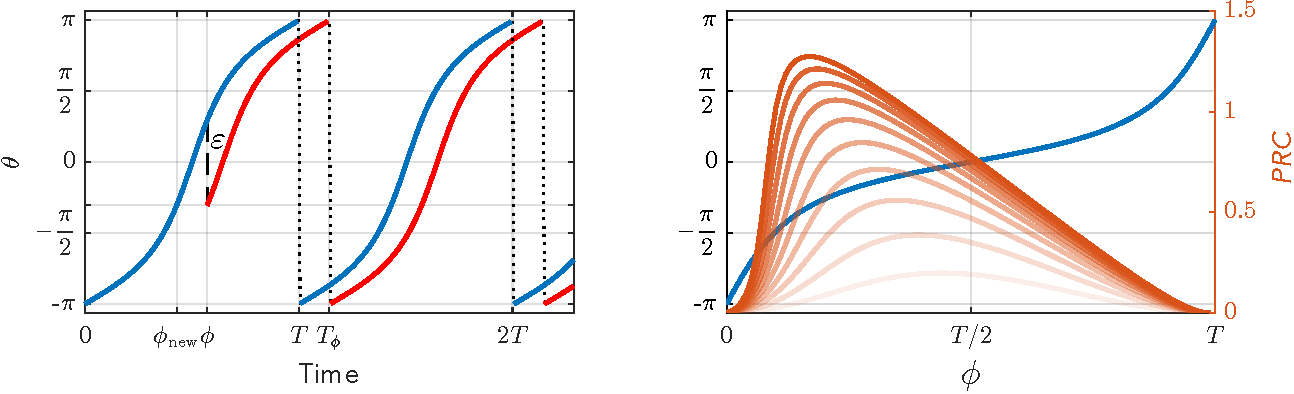
\includegraphics[width = \textwidth]{../Figures/ThetaNeuronPRC.pdf}
\caption{Response of the Theta model to bifurcations on the phase. Left: a bifurcation $\varepsilon  < 0 $ at time $\phi$ perturbs $\theta(t)$ (in blue) which results in a delayed spike (trajectory in red), using $I = 5$. Right: The \PRC, \eqref{eq:PRC2} in orange, with a solution for $\theta$ (in blue), to show when the model is the most susceptible to bifurcations over the course of one period, using $I = 0.1$.}
\label{fig:ThetaNeuronfIPRC}
\end{figure}



% !TEX root = ../main.tex
\newpage
\section{Network Topologies} \label{sec:NetworkTopologies}

Networks consists of \textsl{nodes} $n_j$, $j \leq N$ connected by \textsl{links}. They arise in any context where objects are \textsl{related} to each other. 

\subsection{Representations and properties}
We represent a finite network through the adjacency matrix: $A_{ij} $ = 1 if there exists a relation from node $j$ to node $i$ and 0 otherwise. This means that $A_{ij}$ can be \textsl{undirected} (symmetric) or \textsl{undirected}. If we think of the relations between guests at a party, then the social network is directed, as people might not know each other mutually. However, the network of people having shaken hands is symmetric. Self-links are an edge-case that depends on the context, as one generally does not shake hands with himself. \\
%The number of links that a node has is denoted as the \textsl{degree}. 
From $A_{ij}$ we can compute the in- and out-degree vectors, which show how many links a node has coming in and out:
\begin{align}
\kinbi = \sum_{j=1}^{N} A_{i j} \hspace{15mm} \koutbj = \sum_{i=1}^{N} A_{i j}  \hspace{15mm} \degree(n_j) = \k_j = (\boldsymbol{k}_j^{\bf in}, \koutbj) \in \K \subset \mathbb{N} \label{eq:definekinkoutfromA} 
\end{align}
The distribution of $\kinb$ and $\koutb$ is the most defining property of the network:
\begin{align}
(\kinb, \koutb) \sim P(\degree(n) = \k) \label{eq:definekinkoutfromP} \end{align}
The support of $P$ is the set of unique degrees $\K$ with cardinality $M_\k$, which consists of integers. For symmetric networks, $\kinb = \koutb$, so that $P$ is really a univariate distribution.

\subsection{Fixed-degree networks}
\noindent A network consists of nodes, connected by links. The most simple network is one where all the nodes are connected, and so all nodes have a degree of $N$. In general, we can make networks where all nodes have the same degree, $\kmean$:
\begin{align}
P(k) = \left\{\begin{array}{ll}\kmean & \text{if } k=\kmean \\0 & \text{otherwise}\end{array}\right. \hspace{15mm} \K = \{ \kmean \} \label{eq:diracpdf}
\end{align}
We will refer to these networks as fixed-degree networks.


\subsection{Random / Erd{\"o}s-R{\'e}ny networks}
In 1959 Erd{\"o}s and R{\'e}ny published their work on random graphs\cite{RandomGraphs1959}, where links are established if a random uniformly distributed number is higher than a threshold $p$. The degrees follow a binomial distribution: 
\begin{align}
P(k)=\left(\begin{array}{c}N-1 \\ k\end{array}\right) p^{k}(1-p)^{N-1-k}  \hspace{15mm} \K = [0,N] \label{eq:binomialpdf}
\end{align}
with a mean $\mu = p(N-1)$ and standard deviation $\sigma = \mu(1-p)$. For networks where $\kmean \ll N$, the network can be well approximated by a Poisson distribution:
\begin{align}
P(k) = e^{-\kmean} \frac{\kmean^{k}}{k !} \hspace{15mm} \K = [0,N] \label{eq:poissonpdf}
\end{align}
with a mean $\mu = \kmean$ and standard deviation $\sigma = \sqrt{\kmean}$. Both \eqref{eq:binomialpdf} and \eqref{eq:poissonpdf} describe similar quantities, but the latter is used more often due to its analytical simplicity \cite{BarabasiNetworkBook2016}.


\subsection{Scale-free networks}
What we can often observe in nature is the preferential attachment to nodes with a high degree \cite{Bullmore2010}: the rich or famous tend to get more rich or famous. This trait is also described as the 80/20 rule by Pareto. Networks with this property consist of a small number of highly connected nodes, and a large number of low degree nodes. We can represent this with a power law distribution:
\begin{align}
P(k) = A k^{-\gamma} \label{eq:scalefreepdf}
\end{align}
with $A$ is a constant so that $\sum_{k=1}^{\infty} P(k) = 1$. We can also see that $A \sum_{k=1}^{\infty} k^{-\gamma} = 1$ so that $A = \sum_{k=1}^{\infty} k^{\gamma} = 1/\zeta(k)$, the Riemann Z{\'e}ta function \cite{BarabasiNetworkBook2016}. 

Networks with a distribution like \eqref{eq:scalefreepdf} are called \textit{scale-free} networks, as they lack an internal scale to represent the magnitude of the network: we can observe \eqref{eq:scalefreepdf} on different scales like the probability of two Hollywood actors appearing in a movie, or the connections between web pages on the internet \cite{Barabasi2003}. One description that comes close is the \textit{natural cutoff} $k_{\text{max}}$, the expected degree of the largest degree in the network. As we only expect the largest hub to be the only hub in the domain $[k_{\text{max}}, +\infty]$:
\begin{align*}
\int_{k_{\text{max}}}^{\infty} P(k) dk=\frac{1}{N}
\end{align*}
For \eqref{eq:scalefreepdf} this results in:
\begin{align}
\kmax = \kmin \cdot N^{\frac{1}{\gamma-1}} \label{eq:scalefreecutoff}
\end{align}
which shows that there might be large differences in size between the nodes. There are constraints on $\gamma$ to yield a scale-free network. When $0 < \gamma < 2$ the largest hub grows faster than $N$, so once its degree exceeds $N-1$ there are no more new nodes to connect to. A rigorous proof is given in \cite{Bassler2011}. For $\gamma = 2$, the system grows linearly, as we can see in \eqref{eq:scalefreecutoff}. When $2 < \gamma \leq 3$ we find the most scale-free networks, as for $\gamma > 3$ hubs are not sufficiently large and numerous to have much influence on the network
\cite{BarabasiNetworkBook2016}.

% !TEX root = ../main.tex
\newpage
\section{\theory Mean Field Reductions} \label{sec:MFRs}
The \textsl{mean-field reduction} (\MFR) is a theory that can predict the dynamics of the order parameter \eqref{eq:orderparameter}. In \cite{OttAntonsen2008, OttAntonsen2009, OttAntonsen2010} such a method was published for fully connected networks of indistinguishable oscillators with harmonic coupling. In \cite{Restrepo2014} the authors extended their work to include networks with arbitrary degree distributions, applied to the Kuramoto model. Later this analysis was extended to networks of the Theta Neuron model \cite{OttAntonsen2017}. We will now consider the limit $N \gg 1$ and formulate an exact \MFR for different types of networks, following the method in \cite{OttAntonsen2017}. 

\subsection{The Ott-Antonsen manifold}
To simplify notation, the authors incorporate the network size in to $P$ so that $\sum_{\k \in \K} P(\k) = N$. To specify the probability of a link from a node of degree $\kacc$ to one of degree $\k$ we can define an assortativity function:
\begin{align}
a\left(\k_j \rightarrow \k_i \right) = 0 \leq \frac{k^{\rm{out}^{\prime}}_j k^{\rm{in}}_i}{N \kmean} \leq 1 \label{eq:assortativityfunction}
\end{align}
where we have chosen a neutral assortativity \cite{OttAntonsen2017}. \eqref{eq:assortativityfunction} is constrained so that the number of links in the network, $N \kmean$, remains constant \cite{Restrepo2014}:
\begin{align*}
\sum_{\kacc \in \K} \sum_{\k \in \K} P\left( \kacc \right) \: a\left(\kacc \rightarrow \k\right) P\left(\k\right) = N \kmean
\end{align*}
We can now assume that the state of all neurons can be represented by a probability density function $f(\theta, \eta | \k, t)$. Hence, the marginal distribution 
\begin{align*}
    \int_{\R} \int_{\mathbb{I}} f(\vartheta, \eta^{\prime} | \k, t) \mathop{d \vartheta} \mathop{d \eta^{\prime}} 
\end{align*}
gives the fraction of nodes of degree $\k$ with a phase in $\mathbb{I} \subset \T$ at time $t$. Also, we assume $\eta_i$ do not change over time, so that $\int_{\T} f(\vartheta, \eta^{\prime} | \k, t) \: \mathop{d \vartheta}$ yields the excitability distribution $g(\eta | \k)$. \\

To describe the global synchronisation of the network of theta neurons \eqref{eq:thetaneuronnetwork} we have introduced the order parameter $Z(t)$\eqref{eq:orderparameter}. It is now hypothesized that $Z(t)$ can be approximated by a mean-field order parameter, defined by the continuum limit:
\begin{align}
\bar{Z}(t)= \frac{1}{N} \sum_{\k \in \K}P(\k) \int_{\R} \int_{\T} f\left(\vartheta, \eta^{\prime} | \k, t\right) e^{\ic \vartheta} \mathop{d \vartheta} \mathop{d \eta^{\prime}} \label{eq:meanfieldorderparameter}
\end{align}
Here, $f$ is constrained by a continuity equation, as the number of oscillators is conserved:
\begin{align}
\frac{\partial f}{\partial t}+\frac{\partial}{\partial \theta}\left(v_{\theta} f\right) = 0 \label{eq:transportequation}
\end{align}
with $v_{\theta}$ a continuum version of \eqref{eq:thetaneuronnetwork}:
\begin{align*}
v_{\theta} &= (1-\cos \theta)+(1+\cos \theta) \left[\eta + I(\k,t) \right]\\
I(\k,t) &= \frac{\kappa}{\kmean}\sum_{\kacc \in \K} P(\kacc ) \:a\left(\kacc \rightarrow \k \right) \times \left[ \int_{\R} \int_{\T} f\left(\vartheta, \eta^{\prime} | \kacc, t\right) \: a_{2} \left(1-\cos \vartheta\right)^{2} \mathop{d \vartheta} \mathop{d \eta^{\prime}} \right] &
\end{align*}
In \cite{OttAntonsen2008} it is shown that there exists a manifold of invariant probability densities for the continuity equation. The exact \MFR is obtained by expanding $f$ as a Fourier series, and expanding the pulse $\mathcal{P}_s$ using the binomial theorem. When assuming $\eta_i$ is distributed according to a Lorenz distribution:
\begin{align}
g(\eta |\k)=\frac{1}{\pi} \frac{\sigma(\k)}{(\eta-\eta_{0}(\k))^{2}+\sigma(\k)^{2}} \label{eq:Lorentzpdf}
\end{align}
the set of reduced equations then takes a particularly simple form, as \eqref{eq:meanfieldorderparameter} can be evaluated at the poles of $g$ using the Cauchy residue theorem for the integration of complex variables and we find a closed form expression. We can now capture the dynamics by $z(\k,t)$, the mean-field variable for nodes of degree $\k$:
\begin{align}
\frac{\partial z(\k, t)}{\partial t} &= -\ic \frac{(z(\k, t)-1)^{2}}{2} + \frac{(z(\k, t)+1)^{2}}{2} \cdot I(\k, t) \qquad \qquad z \in \C^{M_\k} \nonumber \\
I(\k, t) &= -\sigma(\k) + \ic \eta_{0}(\k) + \ic H_2(\k,t) \label{eq:OttAntonsenSystemFull} \\
H_2(\k,t) &= \frac{\kappa}{\kmean} \sum_{\kacc \in \K} P\left(\kacc\right) \: a\left(\kacc \rightarrow \k\right)  \left( 1 + \frac{z(\kacc, t)^2 + (z(\kacc, t)^c )^2}{6} - \frac{4}{3} \Re(z(\kacc, t)) \right) \nonumber
\end{align}
with $z^c$ the complex conjugate. $H$ is a legacy term and has been computed in \cite{Martens2020}.
The mean-field order parameter can now be expressed in terms of $z(\k,t)$: using the constraints on $f$ and $g$ we can solve \eqref{eq:meanfieldorderparameter} as:
\begin{align}
\bar{Z}(t) &= \frac{1}{N} \sum_{\k \in \K} P(\k) z(\k, t) \qquad \bar{Z} \in \C \label{eq:OttAntonsenMeanField}
\end{align}
which clearly reflects the network architecture through $P(\k)$, as in the limit, this is the number of neurons of degree $\k$ that are present in the network. The mean-field dynamics of the whole network are thus equal to a weighed average of the degree dynamics of each node with unique degree $\k \in \K$. 

We have now formulated the evolution on the invariant manifold by a reduced set of ordinary differential equations. The \MFR is computationally efficient, and in \cite{OttAntonsen2017} many methods for improving this efficiency further are treated.


\subsection{Simplifications for fixed-degree networks}
In the case of a fixed-degree network, every node has $\deg (\theta_i) = (\kmean, \kmean)$ so:
\begin{align*}
    \frac{1}{\kmean} \sum_{\kacc \in \K} P\left(\kacc\right) \: a\left(\kacc \rightarrow \k\right) = \frac{1}{\kmean} N \left( \frac{\kmean \kmean}{N \kmean} \right) = 1
\end{align*}
For any fixed-degree network, \cref{eq:OttAntonsenSystemFull,eq:OttAntonsenMeanField} reduce to a single complex differential equation:
\begin{align}
\dot{Z}(t)= -\ic \frac{(Z-1)^2}{2}+\frac{(Z+1)^2}{2} \left(-\sigma+ \ic\eta_{0}
+ \ic \kappa \left(1+\frac{Z^{2} + (Z^c)^{2} }{6} - \frac{4}{3} \Re(Z)\right)\right) \label{eq:MeanField}
\end{align}
This is an identical formulation as in \cite{Luke2013} and \cite{Martens2020}. For any fixed-degree network, the reduced system is thus a complex (two-dimensional) system with three bifurcation parameters $\eta_0, \sigma$ and $\kappa$, \cite{Luke2013, Martens2020}. We will start our analysis with \eqref{eq:MeanField}.\\

Three distinct macroscopic states can be identified. In the partially synchronous rest state (\PSR) we can observe in Figure \ref{fig:MFRPSR}, $Z$ settles onto a stable node. Most neurons can be found in a resting state $\eta_0 + \sigma \lesssim 0$, and inhibit one another through $\kappa < 0$. Most neurons are therefore inactive, though some spiking neurons from the tail of $g$ are present but have a neglegible effect. \\

In Figure \ref{fig:MFRPSS} we can observe the partially synchronous spiking (\PSS) state, where we can see how $Z$ settles onto a stable focus. This happens predominantly when $\eta_0 - \sigma \gtrsim 0$ and most neurons inherently spike, with the coupling being either excitatory or weakly inhibitory. Although most neurons are active, the network is partially synchronous and organized such that phase cancellation occurs by continuous spiking among the neurons.\\

Lastly, in the collective periodic wave state (\CPW) we can observe a limit cycle of the mean field, in Figure \ref{fig:MFRCPW}. Most neurons are active and inhibitory: $\eta_0 > 0$ and $\kappa < 0$. The collective oscillation emerges from the interplay between the neurons’ inherent tendency to spike and the strong suppressive network interaction. \CPW states are mediated through Hopf bifurcations and homoclinic bifurcations of $Z$. We can also see the occurrence of a saddle-node bifurcation in the lower hand corner, for low $\sigma$. We will continue to study the \CPW due to its interesting properties.\\

A more detailed discussion of the different regimes and bifurcations can be found in \cite{Luke2013}.

% \textcolor{red}{QUESTION}: \textsl{I have worked on the analysis presented in \cite{Luke2013} to make my own figures on the bifurcations. However, I cannot seem to get them plotted. Should I continue on this?}

\begin{figure}[H]
\centering
\begin{subfigure}[b]{0.32\linewidth}
   \centering
  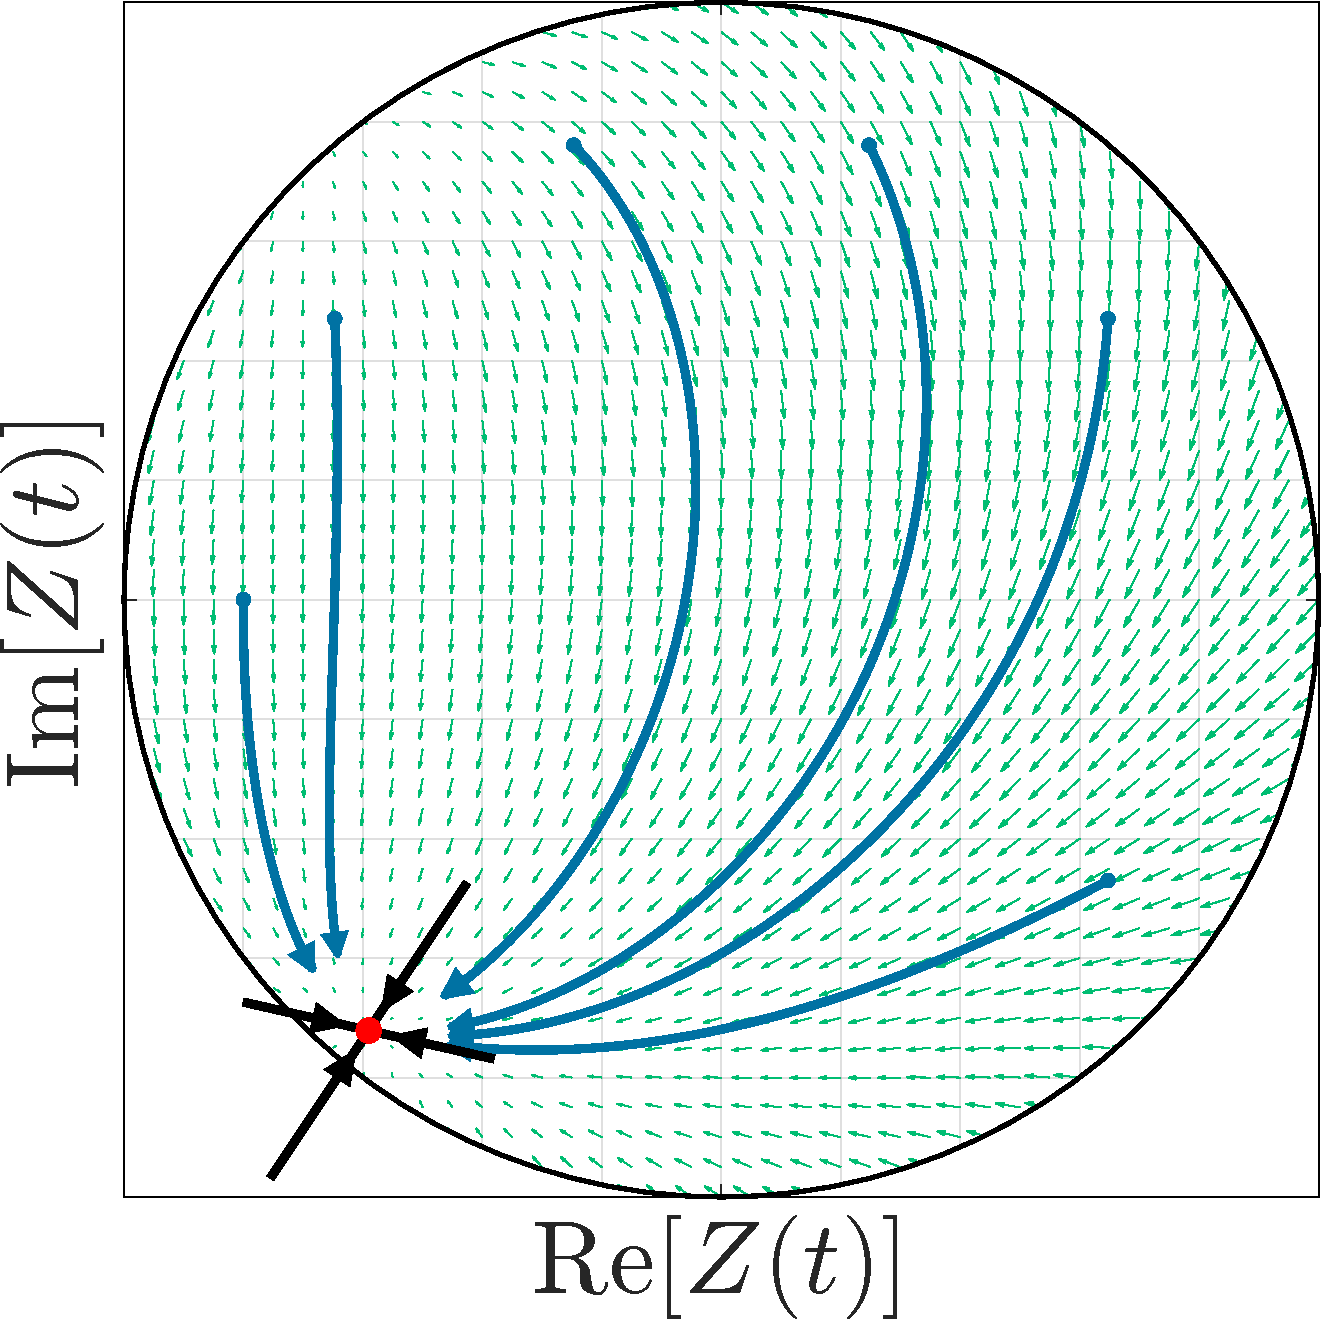
\includegraphics[width=\linewidth]{../Figures/PhaseSpace/MFRPSR.pdf}
   \caption{PSR state for $\eta_0 = -0.9, \sigma = 0.8$ and $\kappa= -2$. The mean field settles onto a stable node.}
   \label{fig:MFRPSR} 
\end{subfigure} \hfill
\begin{subfigure}[b]{0.32\linewidth}
   \centering
  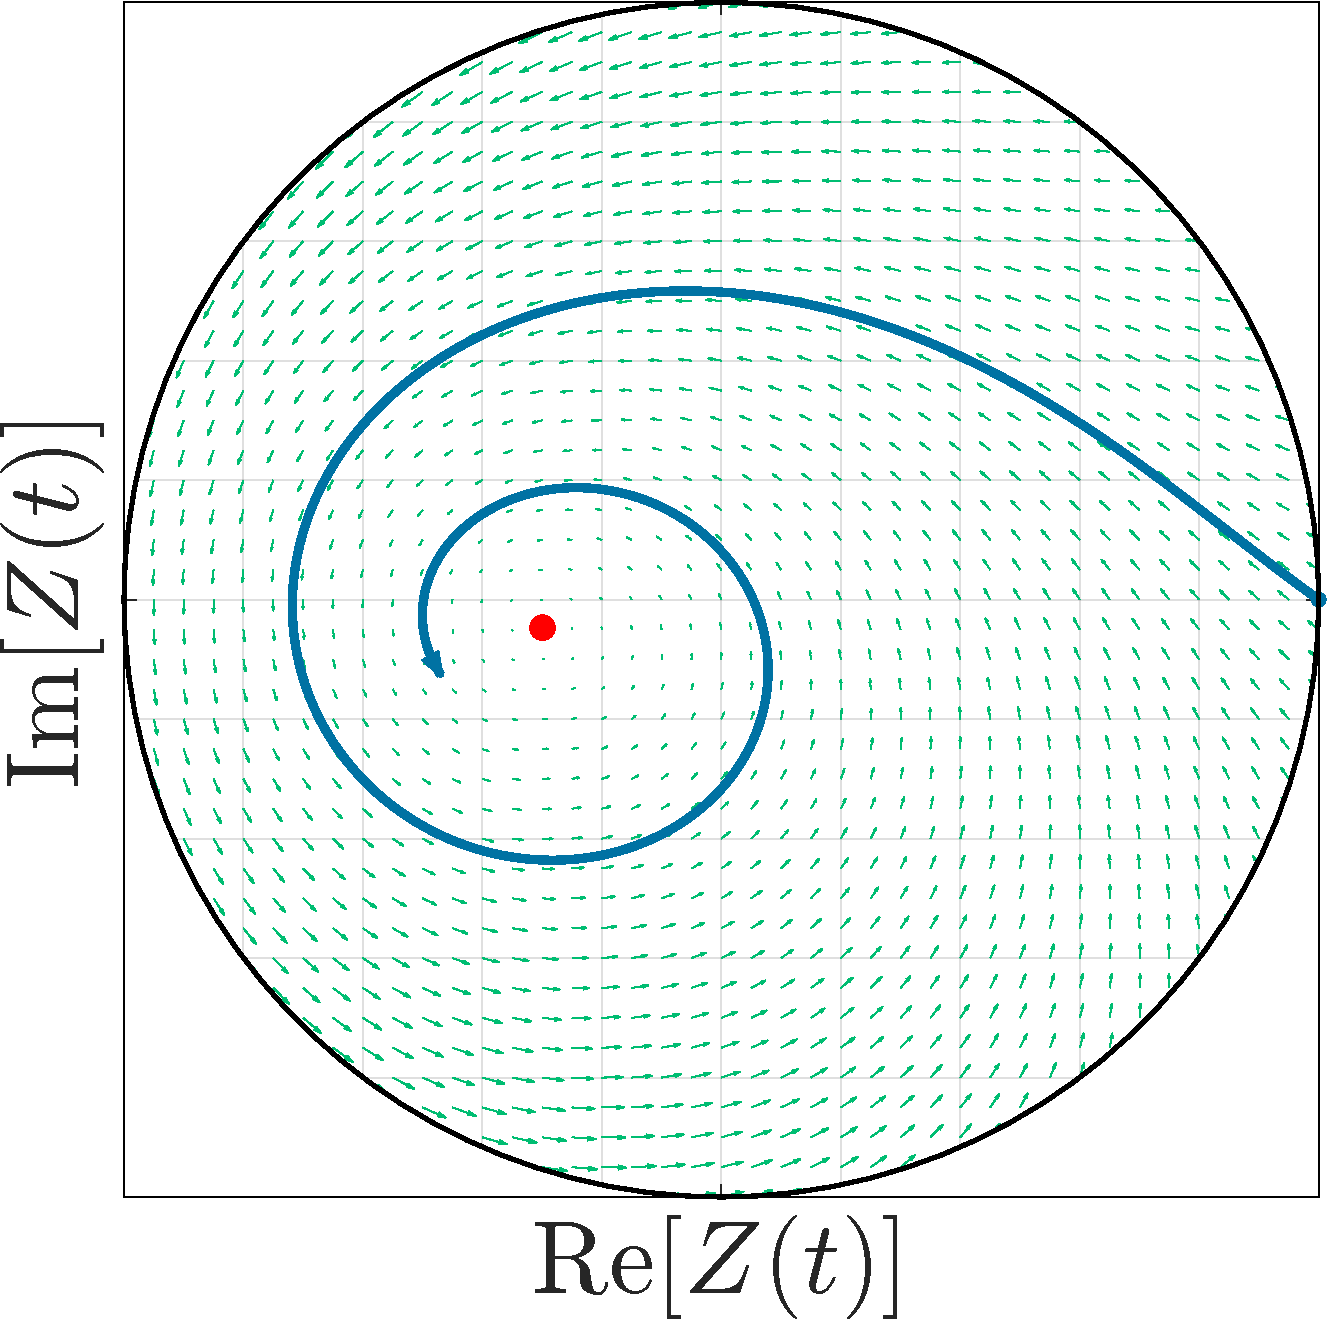
\includegraphics[width=\linewidth]{../Figures/PhaseSpace/MFRPSS.pdf}
   \caption{PSS state for $\eta_0 = 0.5, \sigma = 0.7$ and $\kappa= 2$. The mean field settles onto a stable focus.}
   \label{fig:MFRPSS}
\end{subfigure} \hfill
\begin{subfigure}[b]{0.32\linewidth}
   \centering
  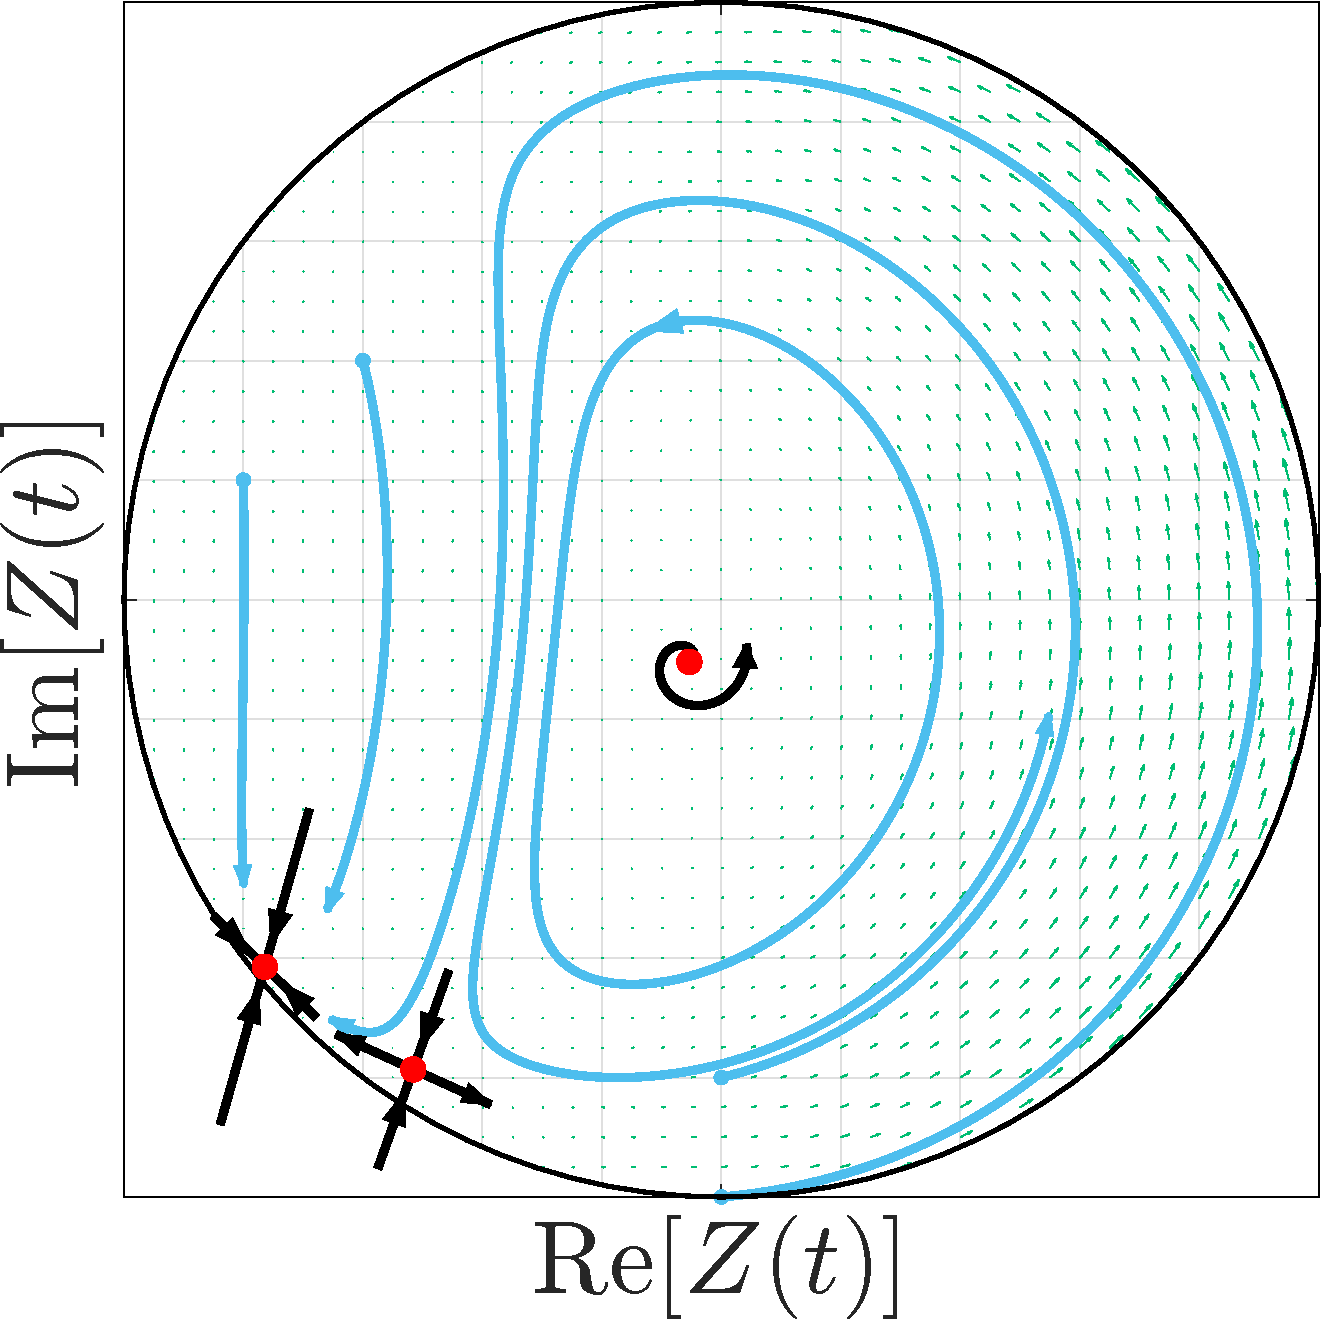
\includegraphics[width=\linewidth]{../Figures/PhaseSpace/MFRCPW.pdf}
   \caption{CPW state for $\eta_0 = 10.75, \sigma = 0.5$ and $\kappa= -9$. The mean field settles onto a stable limit cycle.}
   \label{fig:MFRCPW}
\end{subfigure}
   \caption{Three macroscopic states observed in the \MFR inside the imaginary unit circle $|Z(t)| \leqslant 1$. Green arrows mark the phase space vector field and blue trails mark solution curves. Red points indicate equilibrium points, with black arrows marking the direction of the eigenvectors in that point, scaled according to the magnitude of the corresponding eigenvalues. This information is found from the Jacobian, which we will discuss in Chapter \ref{sec:MFRSUndirected}.}
   \label{fig:macroscopicstatesfixeddegree}
\end{figure}


\subsection{Implications and challenges of the \MFR}
The advantages of using the \MFR can be found in the number of equations we now have left to investigate. As there are $M_{\k}$ equations in \eqref{eq:OttAntonsenSystemFull}, instead of $N$ equations for $N$ neurons, the reduction becomes more and more efficient for larger networks. As we have seen in \eqref{eq:MeanField} this yields a single equation for a fixed-degree network, as all neurons have the same degree.\\

While the \MFR gives us the opportunity to use any arbitray univariate distribution $P(k)$ for undirected, symmetric networks or any bivariate distribution $P(\k)$ for directed, asymmetric networks, none of the publications on the \MFR have treated directed networks. The challenge there is that the support $\K$ is a much larger set, as $\K = \koutb \times \kinb$. For example, the scale-free distribution \eqref{eq:scalefreepdf} has $M_{\k} = \kmax - \kmin$ number of degrees in its support. An example would be $M_{\k} = $ 1250, \cite{OttAntonsen2017}. For 10.000 neurons, that is a reduction of 87,5\%. When we wish to extend \eqref{eq:scalefreepdf} to a bivariate distribution, $M_{\k}$ grows to $\left( \kmax - \kmin \right)^2$. A bivariate distribution would therefore need about $1.56 \times 10^6$ equations for 10.000 neurons. It is not feasible to solve this many equations at once. Even though it is reported that solving only 10\% of the equations and then interpolating across $z$ and $t$ yields a very good approximation of the whole system, \cite{OttAntonsen2017}, the sheer number of equations remains too high.


% !TEX root = ../main.tex
\newpage
\section{\mywork Mean Field Reductions for undirected graphs}
\subsection{Directed graphs as permutations}
So how can we use the \MFR efficiently when the network is a directed graph with an asymmetrical adjacency matrix? Let's investigate.
\begin{itemize}
\item Sampling $\kinb$ and $\koutb$ from a bivariate distribution requires us to find the marginal distribution of $P$ for $\kinb$, sampling $\kinbi$, and then sampling $\koutbj$ from $P$ while keeping $\kinbi$ fixed. This is a cumbersome process. And what relation would there be between $\kinb$ and $\koutb$?
\item However, if we assume that the marginal distributions for $\kinb$ an $\koutb$ are independent, there is a simplification to be found. We can even assume that the two marginal distributions are identical univariate distributions. 
\item Hence, we can sample $\kinb$ from a univariate distribution and find $\koutb = \permute ( \kinb )$ so that the total number of links remains constant. 
\end{itemize}

This hypothesis can be tested: we assume that $P(\k) = P(\kin) \cdot P(\kout)$ so that $P$ consists of two identical and independent distributions, given by the distributions presented in Chapter \ref{sec:NetworkTopologies}. Then, we sample $\kinb \sim P(\kin)$ and perform a permutation to find all node degrees $\k_j$. The surface given by $P$ and the histogram of $\k_j$ have been plotted in Figure \ref{fig:2Ddistributions}. As we can see, the variates follow the distribution well. 

\begin{figure}[H]
\centering
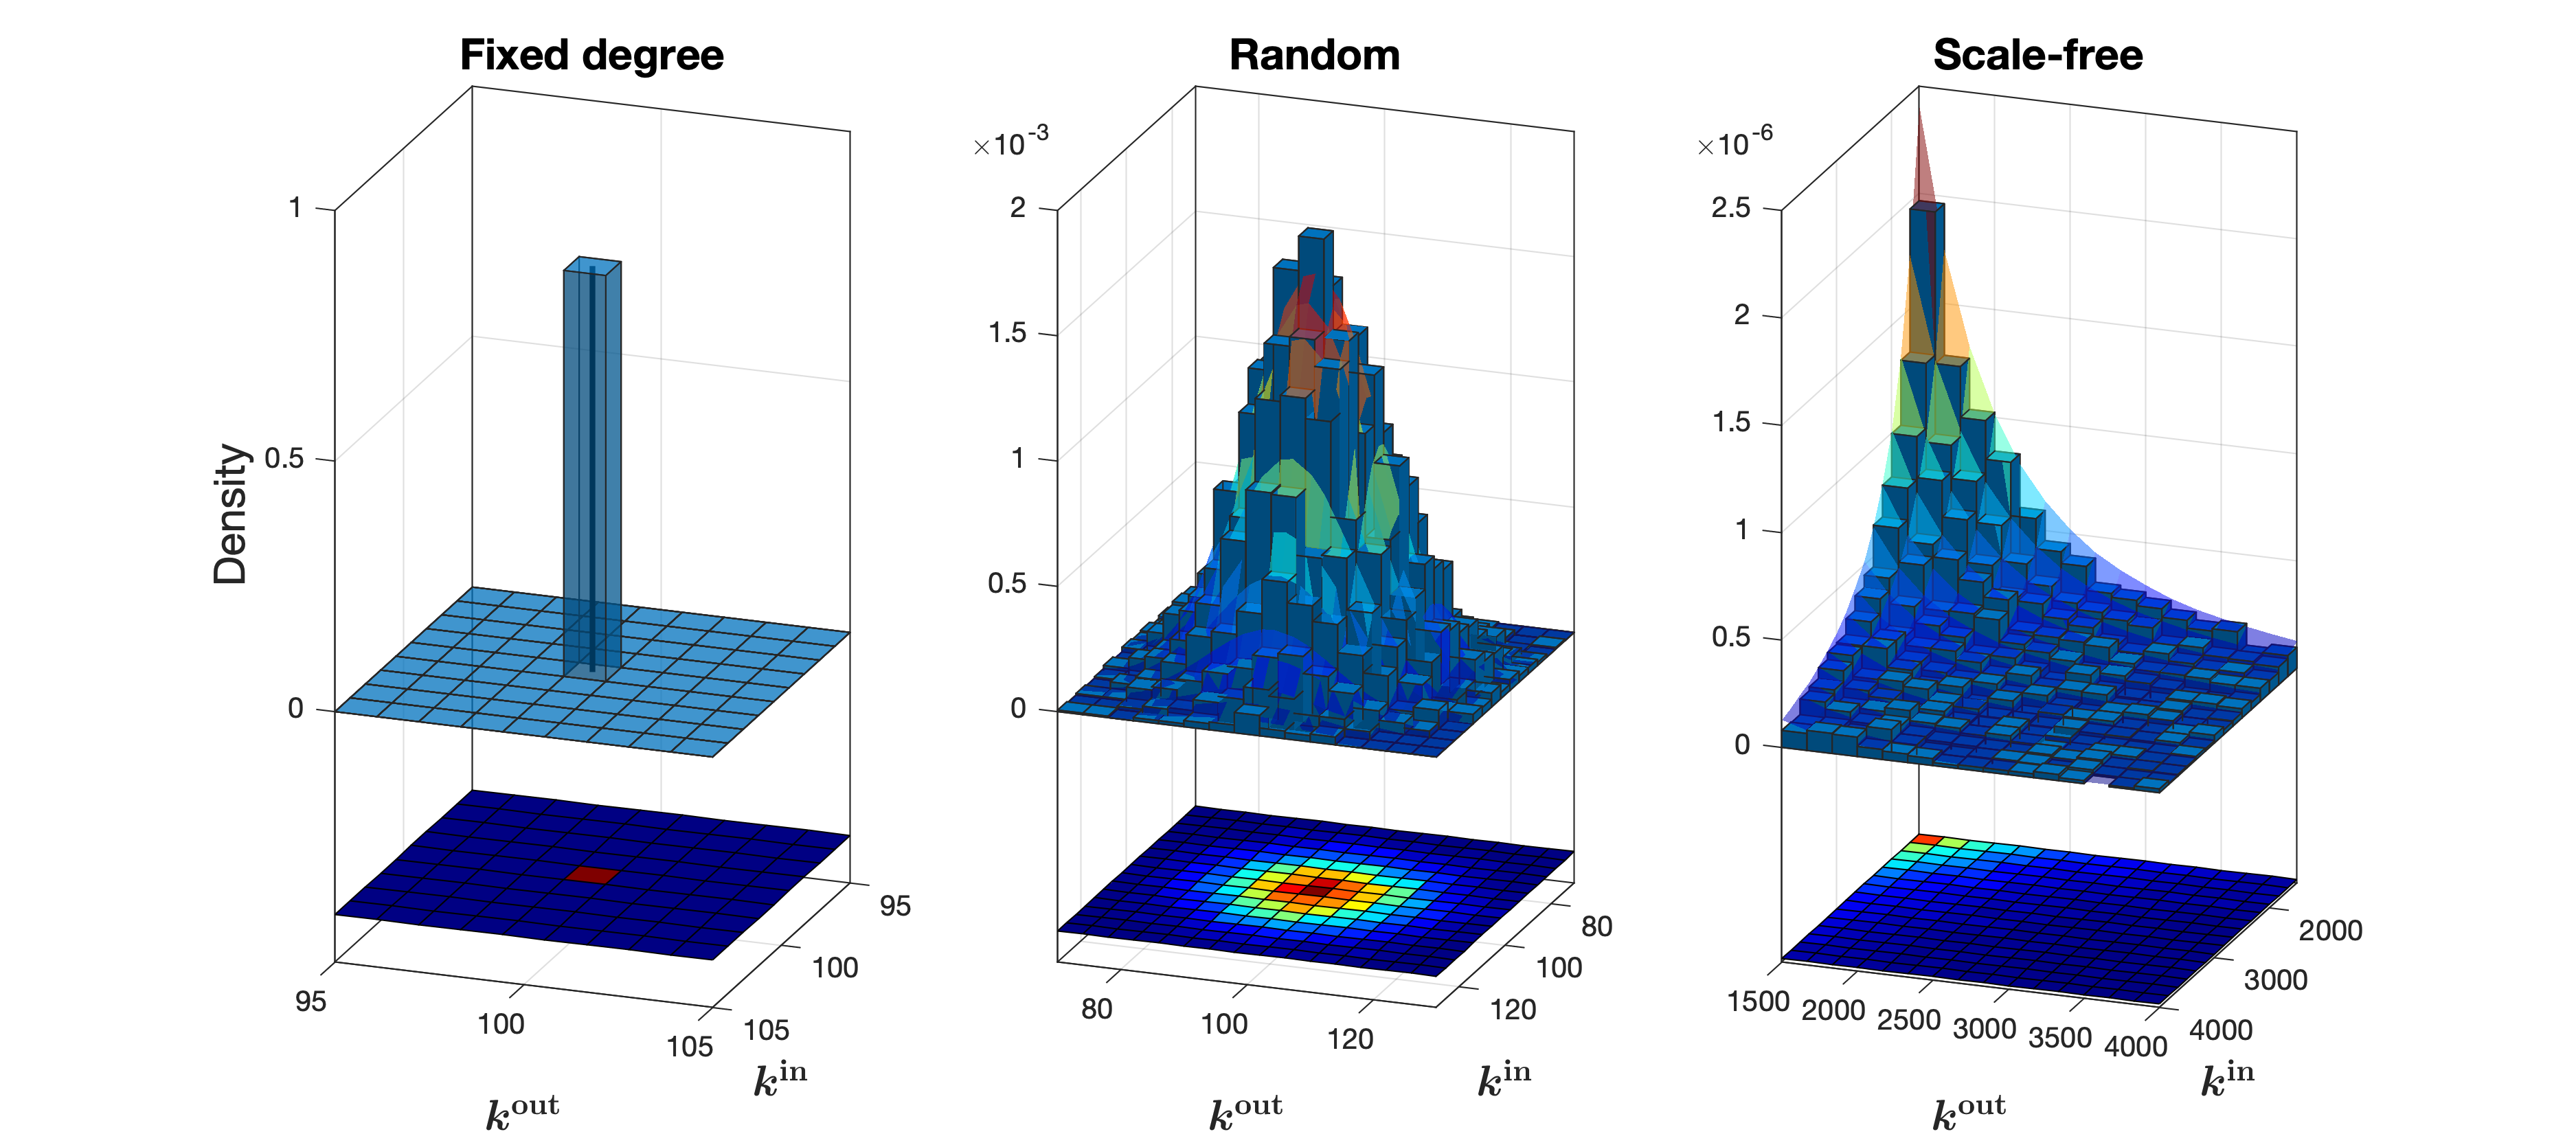
\includegraphics[trim=2.5cm 0cm 2.5cm 0cm, clip=true, width = \textwidth]{../Figures/Distributions/2D.png}
\caption{Bivariate distributions for different network topologies, using 10$^4$ number of samples. The surface given by $P(\k)$ is well approximated by the histogram of variates sampled from a univariate distribution. $\kmean =  2 \times 10^3$ for all topologies, $p \approx 0.2$ for the random network and $\gamma = 4.3$ for the scale-free network.}
\label{fig:2Ddistributions}
\end{figure}


\subsection{Building the adjacency matrix} \label{sec:buildingA}
If we want to simulate the network of theta neurons \eqref{eq:thetaneuronnetworkcurrent} we need to construct the adjacency matrix. We can find an exact solution for $A$ given the degree vectors in \eqref{eq:definekinkoutfromP}. $A_{ij}$ represents a directed graph, but $A_{ij} \neq A_{ji}$ is not a necessary condition. For the elements of $A_{ij}$ we need to find $N^2$ number of variables. We have the following constraints:
\begin{enumerate}
\item The column- and row-sums of $A_{ij}$ must be equal to $\kinb$ and $\koutb$, see \eqref{eq:definekinkoutfromA}. 2$N$ constraints.
\item Self-coupling is mandatory: $A_{ii} = \boldsymbol{1}$. $N$ constraints.
\item The total number of links is constant: $\sum_{i=1}^{N} \kinbi \equiv \sum_{j=1}^{N} \koutbj \equiv \sum_{i,j=1}^{N}A_{i j}$. 1 constraint.
\end{enumerate}
This means that there are $N^2 - (3N + 1)$ variables to find. Once a solution has been found, $A_{ij}$ can be switched with element $A_{ic}$ if $A_{ij} \neq A_{ic}$ and $A_{rj}$ with $A_{rc}$, which yields a new feasible solution. The number of switches one can make is high, and therefore we can simply try a stochastic approach to obtain $A$:
\begin{enumerate}
\item Choose a random row $i \in [1,N]$. $A_{i,i} = 1$, so we need $m = \kinbi - 1$ elements that are 1.
\item Perform $\permute ( \koutbj, j \neq i)$ and therein find the indices $\boldsymbol{\ell}$ of the $m$ first largest elements. 
\item Set $A_{il} = 1 \: \: \forall \: \: l \in \permuteinv (\boldsymbol{\ell})$.
\end{enumerate}
Algorithms that find the largest value in a vector start from the first or the last element. The permutation allows us to find different maxima every time by shuffling the vector.

\begin{figure}[H]
\centering
\begin{subfigure}[b]{0.32\linewidth}
   \centering
  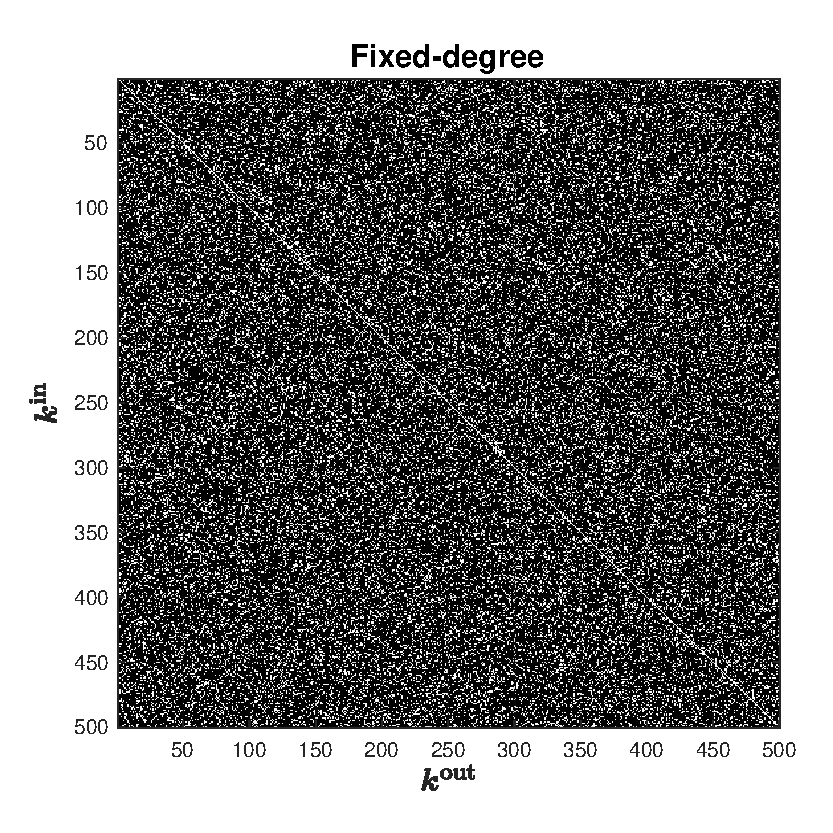
\includegraphics[width=\linewidth, trim={0.5cm 0.5cm 1cm 0.5cm },clip]{../Figures/Adjacency matrices/A_fixeddegree.pdf}
%   \caption{Adjacency matrix for a fixed-degree network.}
 %  \label{fig:A_fixeddegree} 
\end{subfigure} \hfill
\begin{subfigure}[b]{0.32\linewidth}
   \centering
  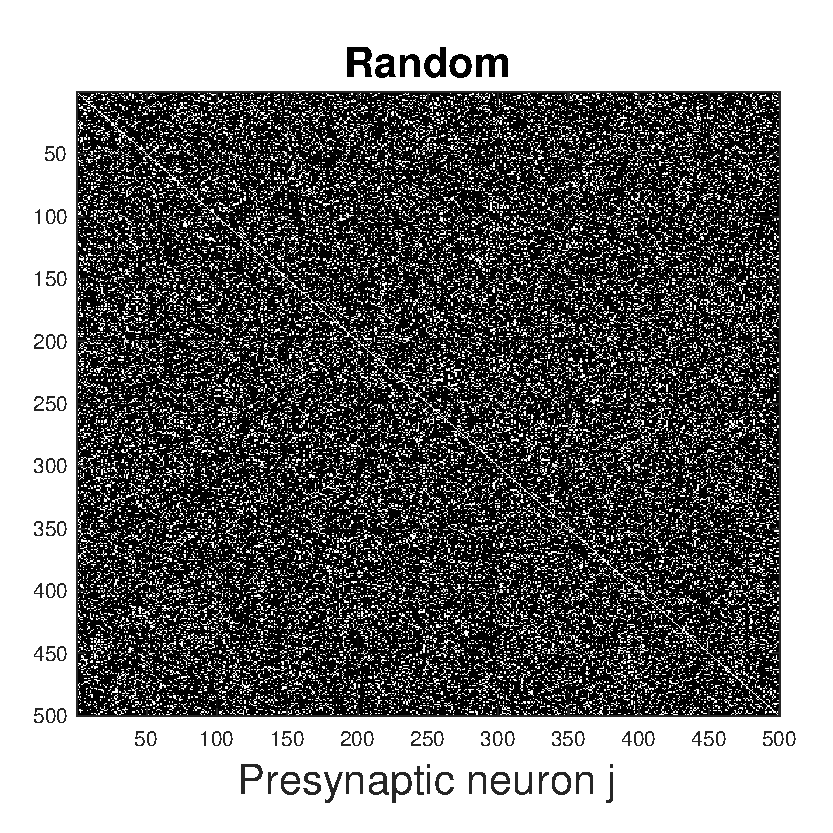
\includegraphics[width=\linewidth, trim={0.5cm 0.5cm 1cm 0.5cm },clip]{../Figures/Adjacency matrices/A_random.pdf}
%   \caption{Adjacency matrix for a fixed-degree network.}
%   \label{fig:MFRPSS}
\end{subfigure} \hfill
\begin{subfigure}[b]{0.32\linewidth}
   \centering
  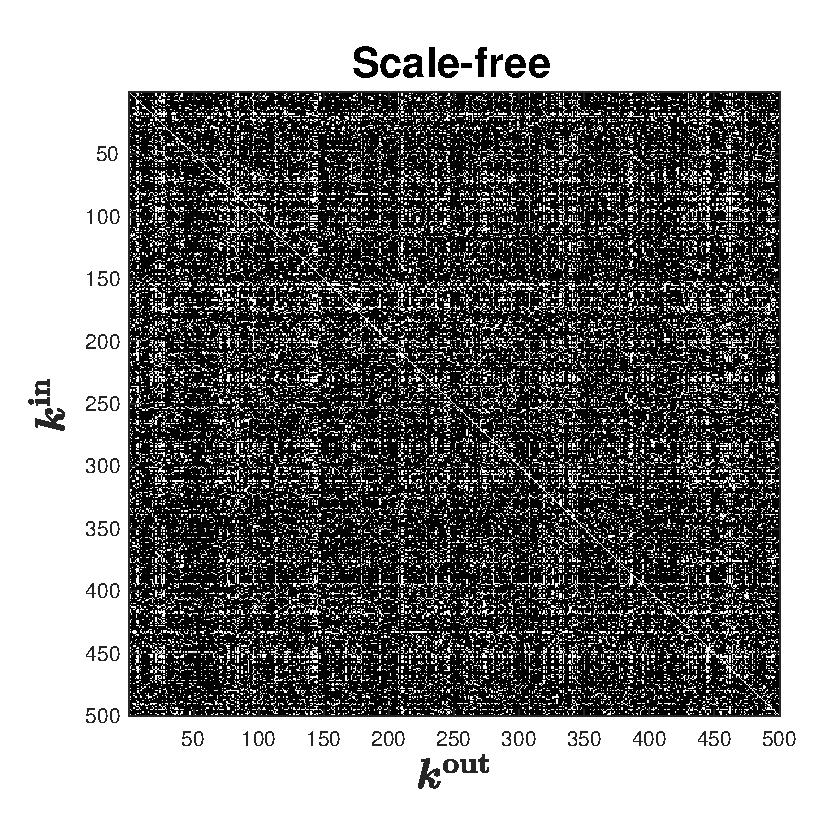
\includegraphics[width=\linewidth, trim={0.5cm 0.5cm 1cm 0.5cm },clip]{../Figures/Adjacency matrices/A_scalefree.pdf}
%   \caption{Adjacency matrix for a fixed-degree network.}
%   \label{fig:MFRCPW}
\end{subfigure}
   \caption{Adjacency matrices for different types of networks with $N$ = 500 and $\kmean$ = 100. We can see how the fixed-degree network is quite homogeneous, while the random network shows some more clustering. The scale-free network has a low number of nodes with a very high degree, which is why we see vertical and horizontal stripes in the adjacency matrix.}
   \label{fig:adjacencymatrices}
\end{figure}


\subsection{Fixed-degree networks as a baseline}
\begin{figure}[H]
\centering
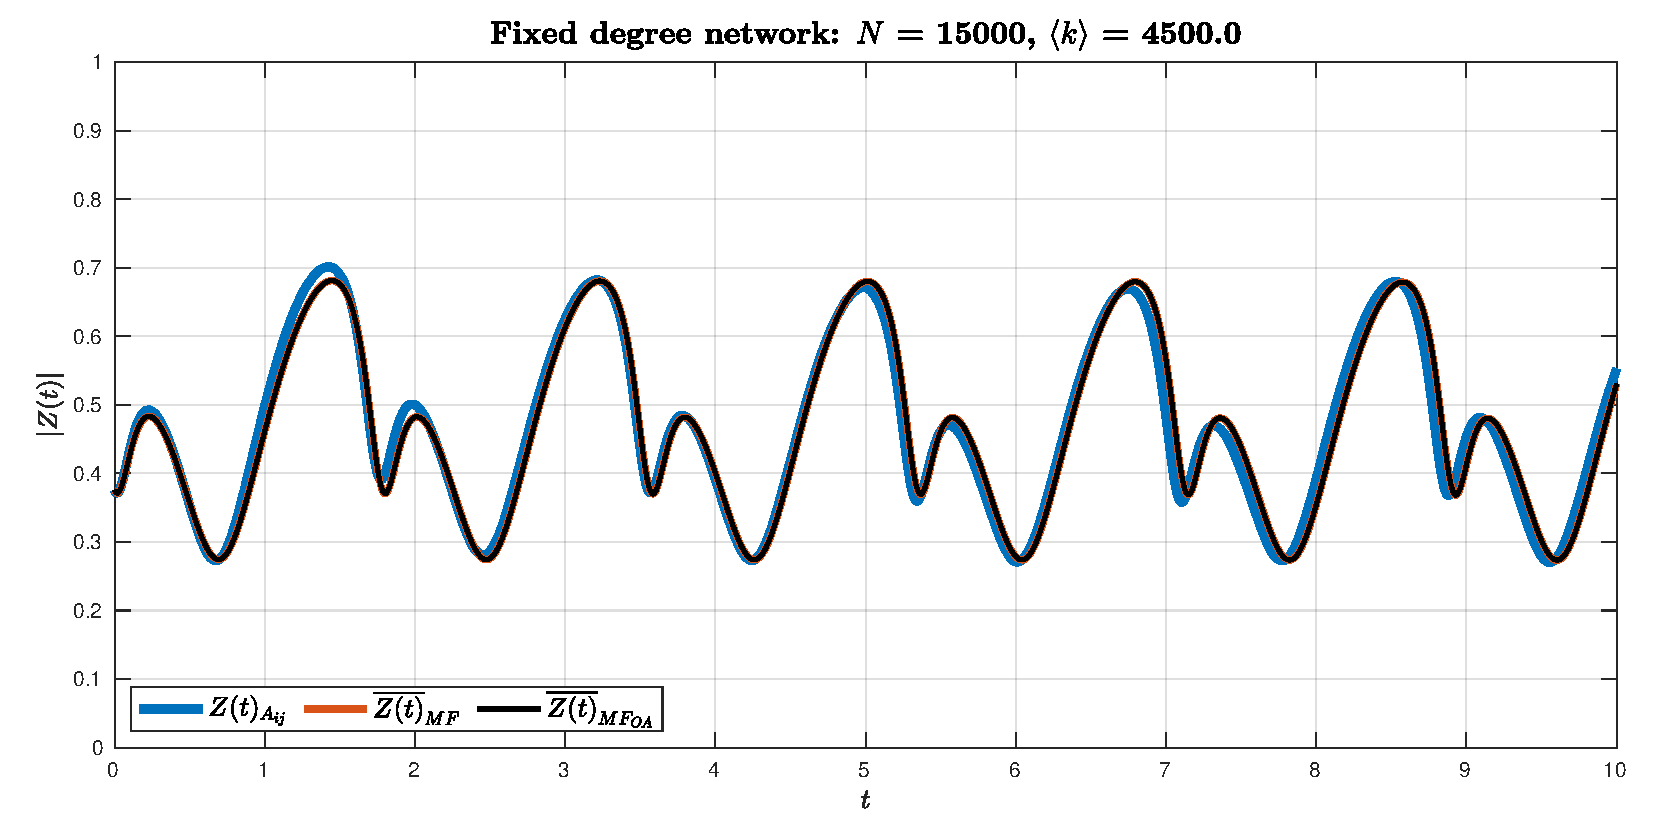
\includegraphics[width = \textwidth]{../Figures/InspectMeanFieldFixedDegree.pdf}
\caption{Comparison}
\label{fig:InspectMeanFieldFixedDegree}
\end{figure}

% !TEX root = ../main.tex
\newpage
\section{Hebbian Learning and Synaptic Plasticity}
\vspace{1mm}
\begin{quote}
\textsl{When an axon of cell A is near enough to excite a cell B and repeatedly or persistently takes part in firing it, some growth process or metabolic change takes places in one or both cells such that A's efficiency, as one of the cells firing B, is increased.}\cite{Hebb1949}
\end{quote}

This quote from Hebb has influenced the neuroscientific community since 1949. In its essence, Hebb postulated that neurons that \textsl{fire together, wire together}. It has since become known as \textsl{Hebbian learning}, and is simply modelled as a positive correlation between the action potentials of spiking neurons. It has been proven in vivo in many studies \cite{ChrolCannon2014}, just like its counterpart, \textsl{anti-Hebbian learning}, where a negative correlation can be found.


\subsection{Spike-timing dependant plasticity}
One specific temporal interpretation of these ideas is \textsl{spike-timing-dependent plasticity} (\STDP), where the relative timing of action potentials from the pre- and postsynaptic neuron determine causality \cite{Kempter1999, Gerstner2002}. If the postsynaptic neuron fires right after the presynaptic neuron, then we can expect the synaptic strength from post- to presynaptic neuron to increase, and vice versa. 

Let us say that neuron $\theta_i$ spikes at time $t_i$ and that neuron $\theta_j$ spikes at $t_j$. Taking the time difference $\Delta t_{ij}$ as $t_j - t_i$, we can say that when $\Delta t_{ij} > 0$ the spikes are correlated (there exists a temporally causal relation), and we can model an increase in synaptic strength of the connection from $\theta_i$ to $\theta_j$, which we will gather in the \textsl{coupling matrix} $K_{ij}$. In the same fashion we can decrease $K_{ji}$ when $\Delta t_{ij} < 0$ as there is no causal relation. 

This means we will find an expression for $\Delta K_{ij}$ in function of $\Delta t_{ij}$ so that at each time-step we can update $K_{ij} \rightarrow K_{ij} + \Delta K_{ij}$.\\

We can think of the coupling matrix as the continuous interpretation of $\kappa A_{ij}$, where synaptic strength and network topology go hand in hand. This also means that we need to redefine some concepts:
\begin{alignat}{2}
\kinbi &= \sum_{j=1}^{N} \rvert K_{i j} \rvert &&\koutbj = \sum_{i=1}^{N} \rvert K_{i j} \rvert \label{eq:definekinkoutfromK} \\
\kmean &= \frac{1}{N} \sum_{i,j=1}^{N} \rvert K_{i j} \rvert \hspace{15mm} && \: \:\hat{\kmean} = \frac{1}{N} \sum_{i,j=1}^{N} K_{i j}  \label{eq:kmeanfromK} 
\end{alignat}
The absolute value ensures that we capture the magnitude of the coupling strength. The reason we want to distinguish between $\kmean$ and $\hat{\kmean}$ is that for some parts of the investigation it is beneficial to study how inhibitive and excitatory coupling strengths influence each other.\\

The functions $W(t)$ that relate $\Delta t_{ij}$ to $\Delta K_{ij}$ are called \textsl{learning windows},  as they define a range in which $K_{ij}$ is able to adapt or \textsl{learn}, and also when learning is optimal. When signals between neurons show a very large time difference (negative or positive) we do not expect them to be correlated. Because the learning windows are generally not symmetrical we can also expect the coupling matrix to be asymmetrical.

Another characteristic is the integral over the learning window. A window with a negative integral directs synaptic strengths mostly towards inhibitory behaviour, and vice versa with a positive integral. An integral of zero would mean that both inhibitory and excitatory synapses are stimulated equally. It has been proven that $\int W(\tau) \mathop{d\tau}$ is the magnitude of the correlation between signals \cite{Gerstner2002}. \\

%The magnitude of change is modulated by an asymmetric biphasic learning window around pulses originating from the postsynaptic neuron. Asymmetric because the peak is not situated at 0 and the integral over the window is generally positive, biphasic because this allows both to strengthen and weaken coupling strengths \cite{Gerstner2002}. 

This approach simplifies modeling the neuronal back-propagation, where another pulse is generated as an echo of the action potential which travels through the neuron dendrites (so, backwards). This behavior is believed to adjust the presynaptic weights, though it is a controversial subject \cite{Gerstner2002}. \\

In recent years, criticism on \STDP has been growing, as experimental data has shown that \STDP is usually accompanied by homeostatic plasticity of the neuron excitability and the synaptic strengths. Processes like \textsl{intrinsic plasticity} (\IP), where one neuron's excitability changes over time as to self-regulate sensitivity to incoming action potentials, or \textsl{synaptic scaling}, where synapse characteristics are adjusted in unison to counteract positive feedback loops, have proven to stabilize the firing rate \cite{ChrolCannon2014, Kirkwood2019}. When \STDP and \IP are combined, it seems like the two process balance each other out and stable network topologies can be found.
%We can model intrinsic plasticity by adjusting the neuron's excitability as the inverse of the firing rate: he more spikes that a neuron will receive, the less affected it is \cite{Song2017}.  An observed phenomenon is that the excitability evolves together with the coupling strength, but that at the extremes this relation reverses \cite{Debanne2017, Debanne2018}.  These types of plasticities should be relatively easy to implement but have no impact on the network topology.


\subsection{Formulations of \STDP as a model}
Following the notation in \cite{Kempter1999}, we will denote the spike train coming from each neuron $\theta_i$ as $S_i^{\rm out}(t) = \sum_{n} \delta (t-t_{i}^{n})$, where $t_{i}^{n}$ is the time that $\theta_i$ has fired. Similarly, we will denote the spike train coming into each neuron $\theta_i$ as $S_i^{\rm in}(t) = \sum_{f} \delta (t-t_{i}^{f})$ with $t_{i}^{f}$ being the time that a neighbouring neuron has spiked. Now we can say that the synaptic strengths are adjusted as:
\begin{align}
\Delta K_{ij} &= \int_{t}^{t+\mathcal{T}} w^{\rm{out}} S_i^{\rm out}(\tau) + w^{\rm{in}} S_{j}^{\rm {in}}(\tau) \mathrm{d}\tau
+ \iint_{t}^{t+\mathcal{T}} W( \tau^\prime - \tau) S_{i}^{\rm out}(\tau) S_{j}^{\rm in}( \tau^\prime) \mathrm{d} \tau \mathrm{d} \tau^\prime
\label{eq:KempterSTDPFormulation1} \\
&= \sum_{t_i^{n}\in \mathcal{T}} w^{\mathrm{out}} + \sum_{t_{j}^{f} \in \mathcal{T}} w^{\mathrm{in}} + \sum_{t_{j}^{f}, t_i^{n} \in \mathcal{T}} W (t_{j}^{f}-t_i^{n} ) \label{eq:KempterSTDPFormulation2}
\end{align}
with $\mathcal{T}$ the period over which learning occurs. $w^{\mathrm{in}} > 0$ and $w^{\mathrm{out}} < 0$ are small weights on the in- and outgoing action potentials and are necessary for $K_{ij}$ to reach an equilibrium. This is proven from the average learning dynamics, \cite{Kempter1999}. In \eqref{eq:KempterSTDPFormulation1} we can recognise the correlation between signals as a convolution over the learning window. \\

The following learning window is proposed:
\begin{align}
W(t)_K = \alpha
\begin{cases}
\left[A_{p}\left(1-\frac{t}{\tilde{\tau}_{p}}\right)+A_{n}\left(1-\frac{t}{\tilde{\tau}_{n}}\right)\right] \cdot \exp \left( \frac{t}{\tau_{\rm syn}} \right) & \text{for } t \leq 0 \\
A_{p} \cdot \exp \left(-\frac{t}{\tau_{p}}\right) + A_{n} \cdot \exp \left(-\frac{t}{\tau_{n}} \right) & \text{for } t > 0
\end{cases} \label{eq:learningwindowKempter1999}
\end{align}
Here $t$ is the delay between presynaptic spike arrival and postsynaptic firing, $\alpha$ is a small learning parameter and all $\tau$ are time constants. Numerical values are usually  $\alpha = 0.05$, $\tau_{\rm syn} = 5$ ms, $\tau_{p} = 1$ ms, $\tau_{n} = 20$ ms and $A_p = 1$ and $A_{n} = -1$. $\tilde{\tau}_{p} \equiv \tau_{\rm syn} \tau_{p} / (\tau_{\rm syn} + \tau_{p})$ and $\tilde{\tau}_{n} \equiv \tau_{\rm syn} \tau_{n} / (\tau_{\rm syn} + \tau_{n})$. \\
$\int W(\tau)_K \mathop{d \tau} = 2.56 \times 10^{-4}$. \\

Using different processes to generate spike trains, the learning equation \eqref{eq:KempterSTDPFormulation2} converges to stable fixpoints. The question will now be whether that is still the case, as changes to the coupling strength will also influence the spiking dynamics between neurons, which in turn will affect the learning again.\\

Another formulation of \STDP as a mathematical model can be found in \cite{Song2000}. It is postulated without being concerned about the biological aspect too much, simplifying some of the ideas of \cite{Kempter1999}. The synaptic strengths are simply updated with:
\begin{align}
\Delta K_{ij} &= K^{\rm max} \cdot \sum_{t_{j}^{f}, t_i^{n} \in \mathcal{T}} W (t_{j}^{f}-t_i^{n} ) \label{eq:SongSTDPFormulation}
\end{align}
where $K^{\rm max}$ is the maximum allowed synaptic strength, so that we can think of \eqref{eq:SongSTDPFormulation} as taking a percentage of the maximum coupling. The authors also constrain $0 \leq K_{ij} \leq K^{\rm max}$. In their further work on \STDP and \IP the authors booked remarkable progress, and their work is very interesting for our application \cite{Song2017}. \\

The learning window is then again defined as a discontinuous function:
\begin{align}
W(t)_S =
\begin{cases}
A_{p} \cdot \exp \left(\frac{-t}{\tau_p}\right) & \text{for } s > 0 \\
A_{n} \cdot \exp \left(\frac{t}{\tau_n}\right)  & \text{for } s \leq 0
\end{cases} \label{eq:learningwindowSong2000}
\end{align}
where we will use $A_p = 0.005$, $A_n = -0.00525$ and $\tau_p = \tau_n = 20$ ms. $\int W(\tau)_S \mathop{d \tau} = -3.70 \times 10^{-4}$ so we expect the weights to be suppressed towards a negative value. 

Recently, triphasic learning windows have been used to account for when it takes too long for the postsynaptic neuron to fire, and thus to decorrelate the relation between neurons. These learning windows are curves that were fitted to experimental data of the cortex and the hippocampus \cite{ChrolCannon2014}. \\

Extending the work of \cite{Song2000} we can find a brief investigation of network topology and clustering using triphasic windows, \cite{ChrolCannon2012}. The method is as in \eqref{eq:learningwindowSong2000}, with the following learning window:
\begin{align}
W(t)_C = A_{p} \cdot \exp \left(\frac{-\left(t - 15 \right)^{2}}{ \tau_{p}}\right) - A_{n} \cdot \exp \left(\frac{-\left(t - 20\right)^{2}}{ \tau_{n}}\right)  \label{eq:learningwindowChrolCannon2012}
\end{align}
where $A_{p}=0.23$, $A_{n}=0.15$, $\tau_{p}=200$ and $\tau_n = 2000$. $\int W(s)_C \mathrm{d}s = -60.0 \times 10^{-4}$.

\begin{figure}[H]
\centering
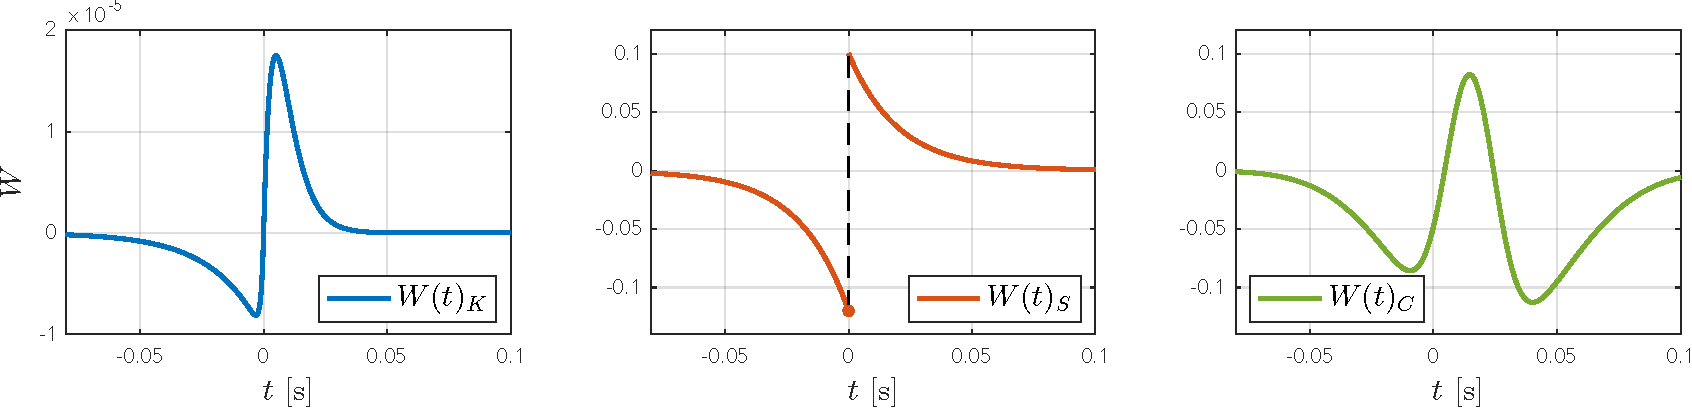
\includegraphics[width = \textwidth]{../Figures/Learning/LearningWindows.pdf}
\caption{Three different biphasic learning windows. Left: in $W_K$ the learning happens much slower, as the magnitude of the window is very small. Middle: we can see how in $W(t)_s$ a larger weight is put on the anti-Hebbian learning. Right: a triphasic window can punish the learning when signals arrive either too early or too late.}
\label{fig:LearningWindows}
\end{figure}

The learning windows generally have $W(t^{\ast}) = 0$ for $t^{\ast} \geq 0$. This means that no learning will take place when the delay between neuron spikes is exactly $t^{\ast} \geq 0$. The triphasic windows show two of those points. 


\subsection{Synaptic scaling}
There is no upper or lower bound on the synapse strength. Also generally, connection strengths are nonzero. This means that the notion of a \textsl{network} is lost.\\
One technique we can apply to keep the strengths within a definitive range is to scale homeostatically - a method where increases in synaptic strength will balance out any decreases by scaling:
\begin{align}
K_{ij}^s = K_{ij} \frac{\frac{1}{N} \sum_{i,j} K_{ij}}{\sum_{i} K_{ij}}
\end{align}
In this way, the out-degrees will remain constant. Using this approach, something has to remain constant, whether that is $\kmean$, or $\kmean^2$ or any other property of the adjacency matrix.


\subsection{Intrinsic plasticity}
Instead of scaling the weights to preserve a certain quantity in the network, we can allow the neurons to adjust their sensitivity to incoming signals. So when some synaptic strengths are increased, we can reduce the excitability, and vice-versa. In \cite{Song2017} such a method is introduced in detail. We can simply update $\eta_{i} \rightarrow \eta_{i} + \eta_{\max } \cdot \phi_{i}$, where: 
\begin{align}
\phi_{i} (t) =
\begin{cases}
-\alpha \cdot \exp \left(\frac{T_{\min }-t}{T_{\rm min }}\right) &\text {for } t<T_{ \rm min } \\ 
\alpha \cdot \exp \left(\frac{t-T_{\rm max }}{T_{\max }}\right) &\text {for } t >T_{\rm max } \\ 
0 &\text {otherwise }
\end{cases}
\end{align}

\begin{figure}[H]
\centering
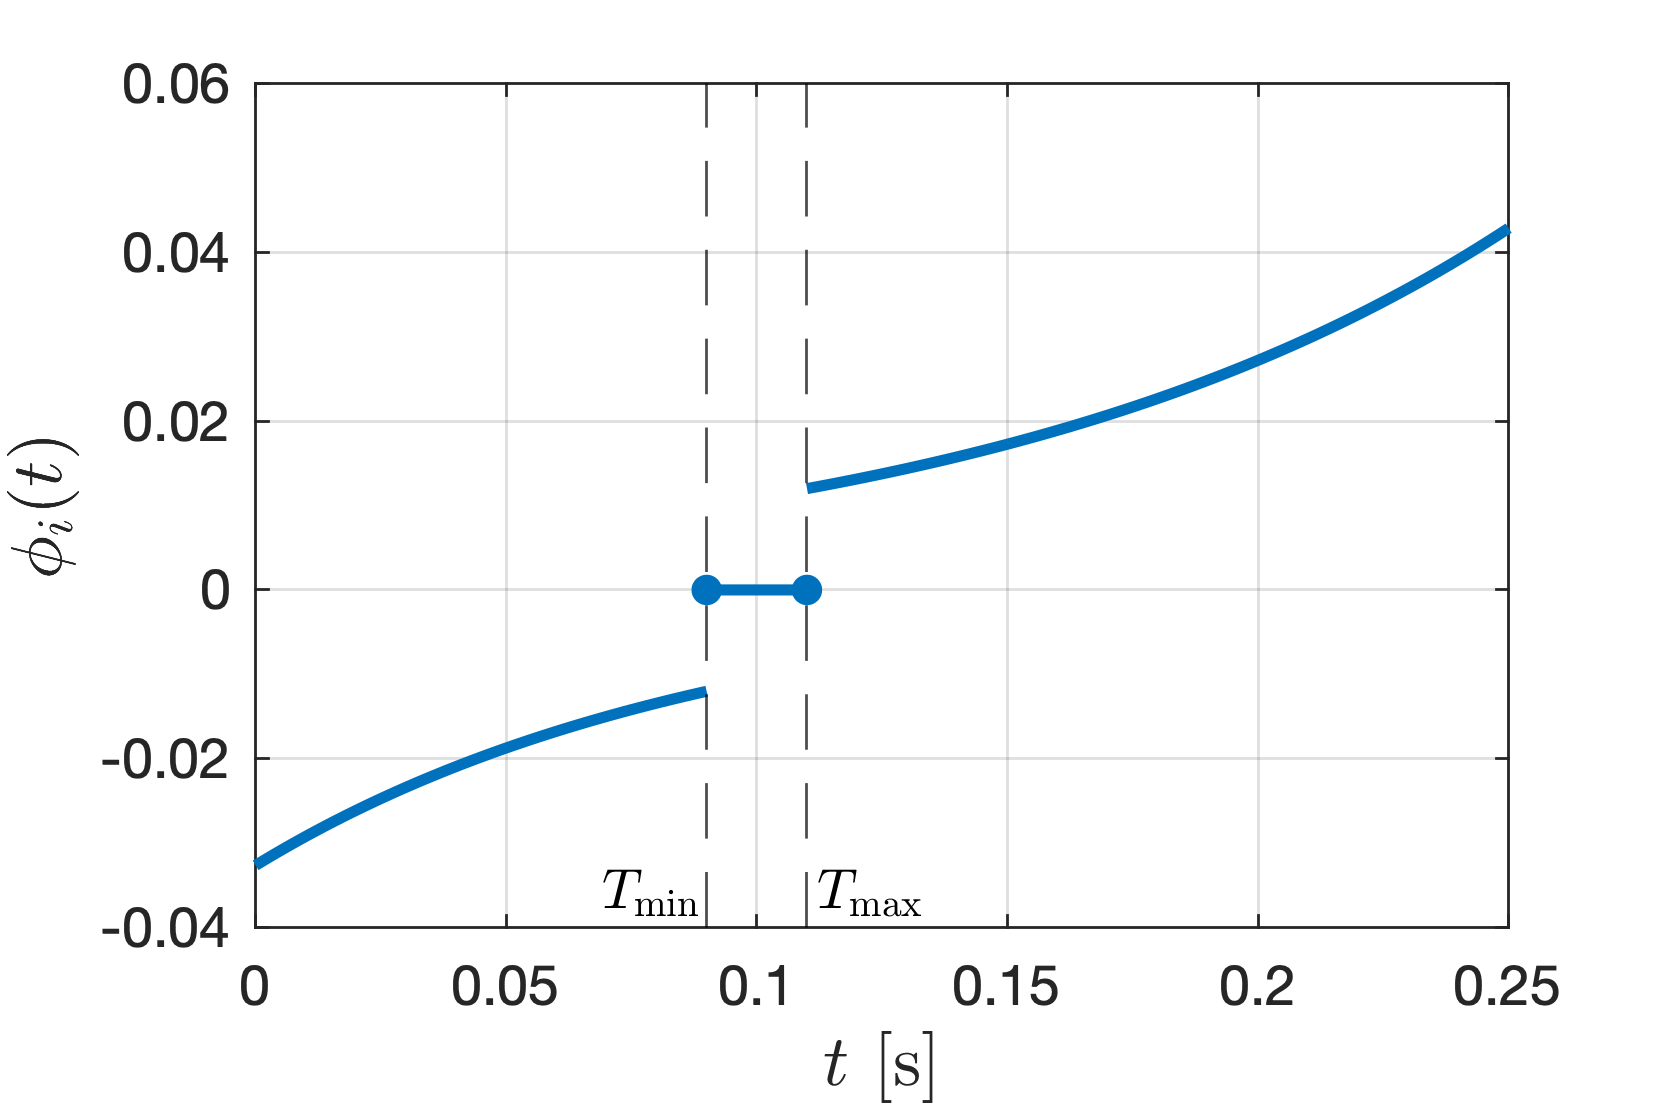
\includegraphics[width = 0.5\textwidth]{../Figures/Learning/IPlearningFunction.png}
\caption{The learning behaviour for intrinsic plastiity as proposed in \cite{Song2017}.}
\label{fig:IPlearningFunction}
\end{figure}


% !TEX root = ../main.tex
\newpage
\section{\mywork Emerging Network Topologies}
\subsection{\STDP applied to networks of theta neurons}
\textcolor{red}{TODO}: \textsl{explain in detail how the different methods \cref{eq:KempterSTDPFormulation2,eq:SongSTDPFormulation} will be implemented, using \STDP coupled with \IP.}

\begin{figure}[H]
\centering
\begin{subfigure}[b]{0.32\linewidth}
   \centering
  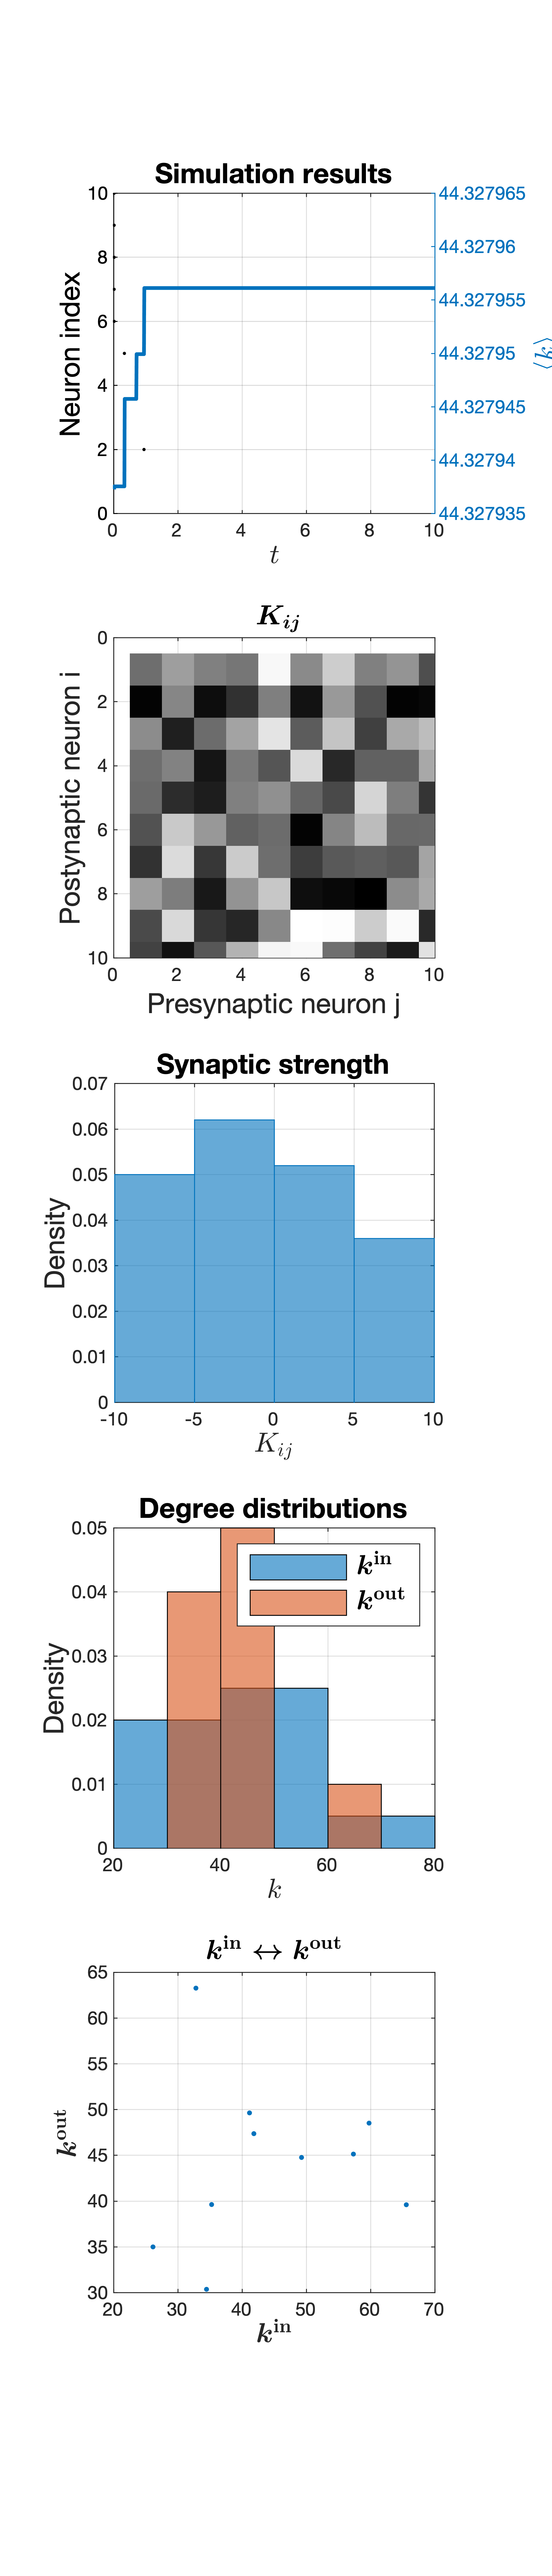
\includegraphics[width=\linewidth, trim={0 0 0 0 },clip]{../Figures/Learning/STDPKempter.png}
   \caption{The window $W_K$.}
   \label{fig:STDPWK} 
\end{subfigure} \hfill
\begin{subfigure}[b]{0.32\linewidth}
   \centering
  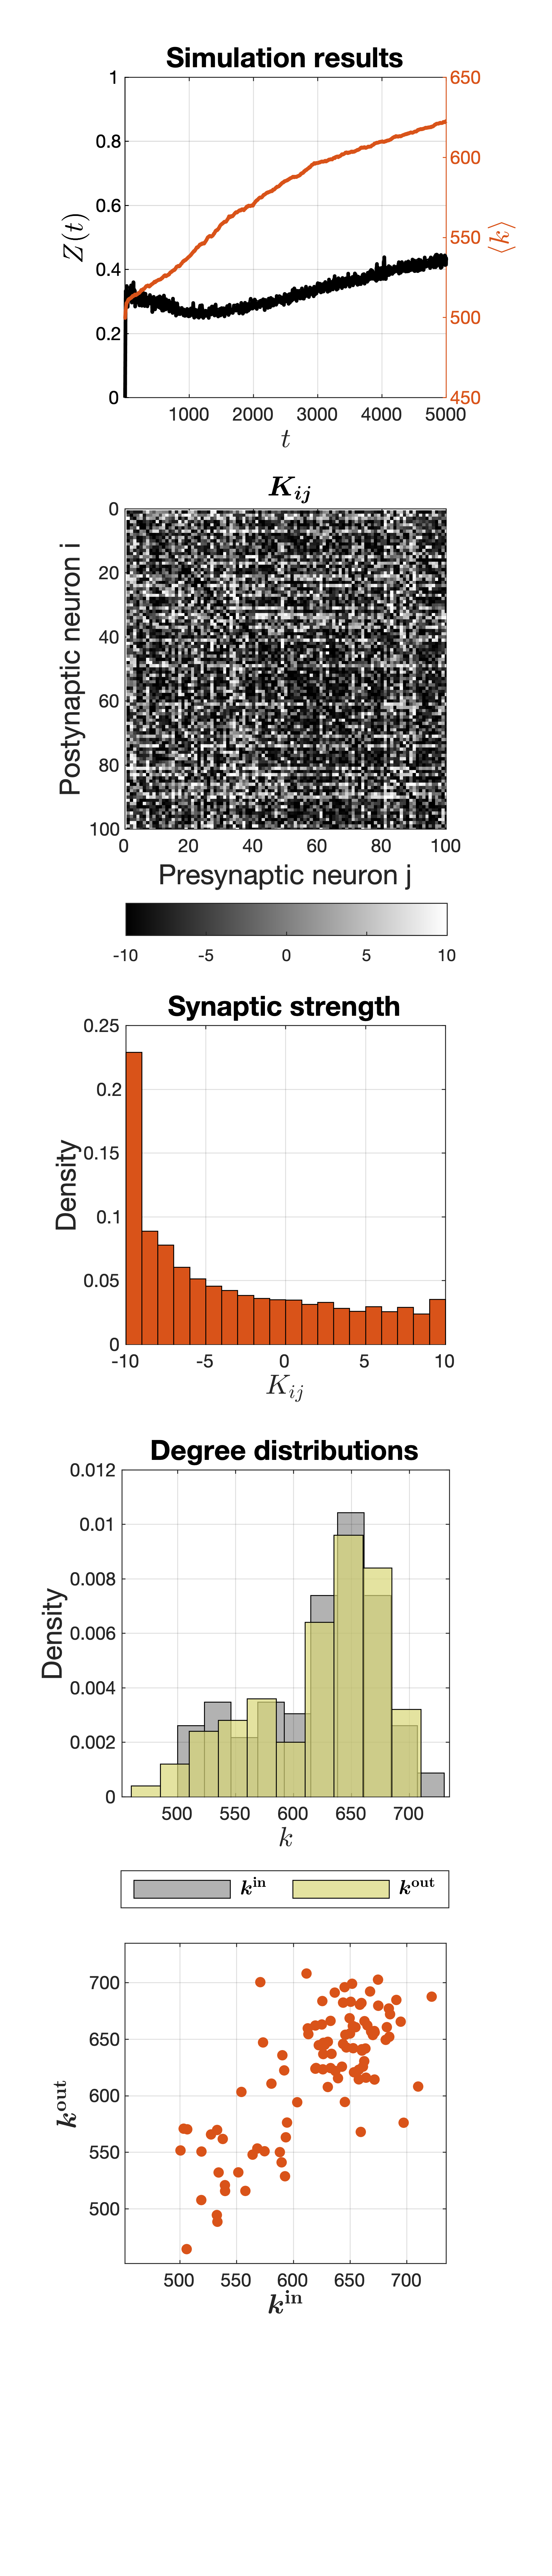
\includegraphics[width=\linewidth, trim={0 0 0 0},clip]{../Figures/Learning/STDPSong.png}
   \caption{The window $W_S$.}
   \label{fig:STDPWS}
\end{subfigure} \hfill
\begin{subfigure}[b]{0.32\linewidth}
   \centering
  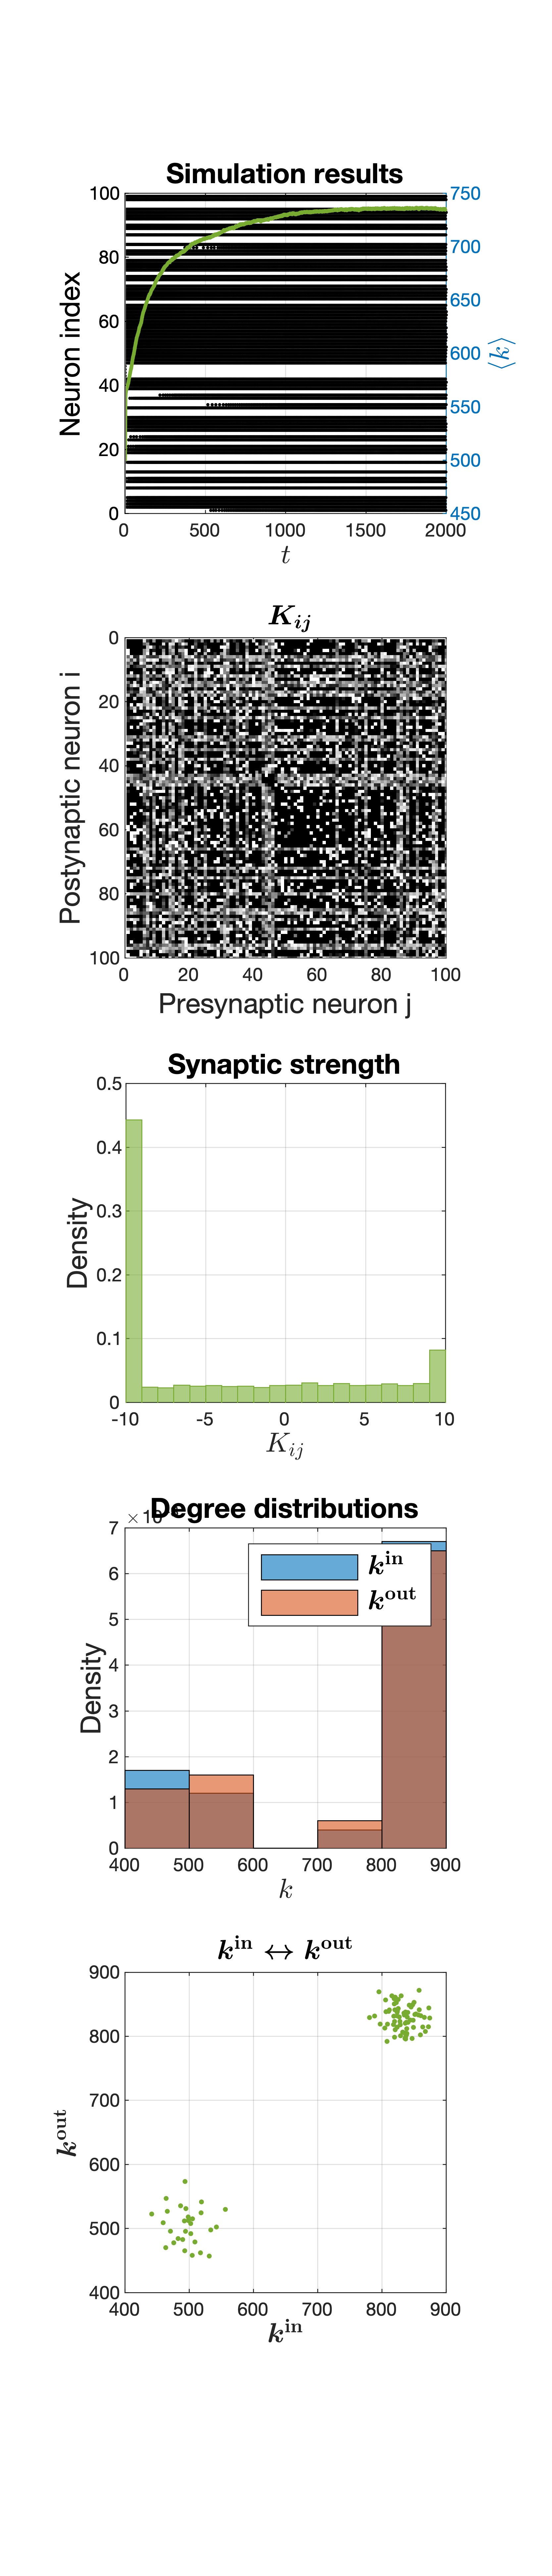
\includegraphics[width=\linewidth, trim={0 0 0 0},clip]{../Figures/Learning/STDPChrolCannon.png}
   \caption{The window $W_C$.}
   \label{fig:STDPWC}
\end{subfigure}
   \caption{Results of the \STDP learning.}
   \label{fig:STDPresults}
\end{figure}

\newpage 

\begin{figure}[H]
\centering
\begin{subfigure}[b]{0.32\linewidth}
   \centering
  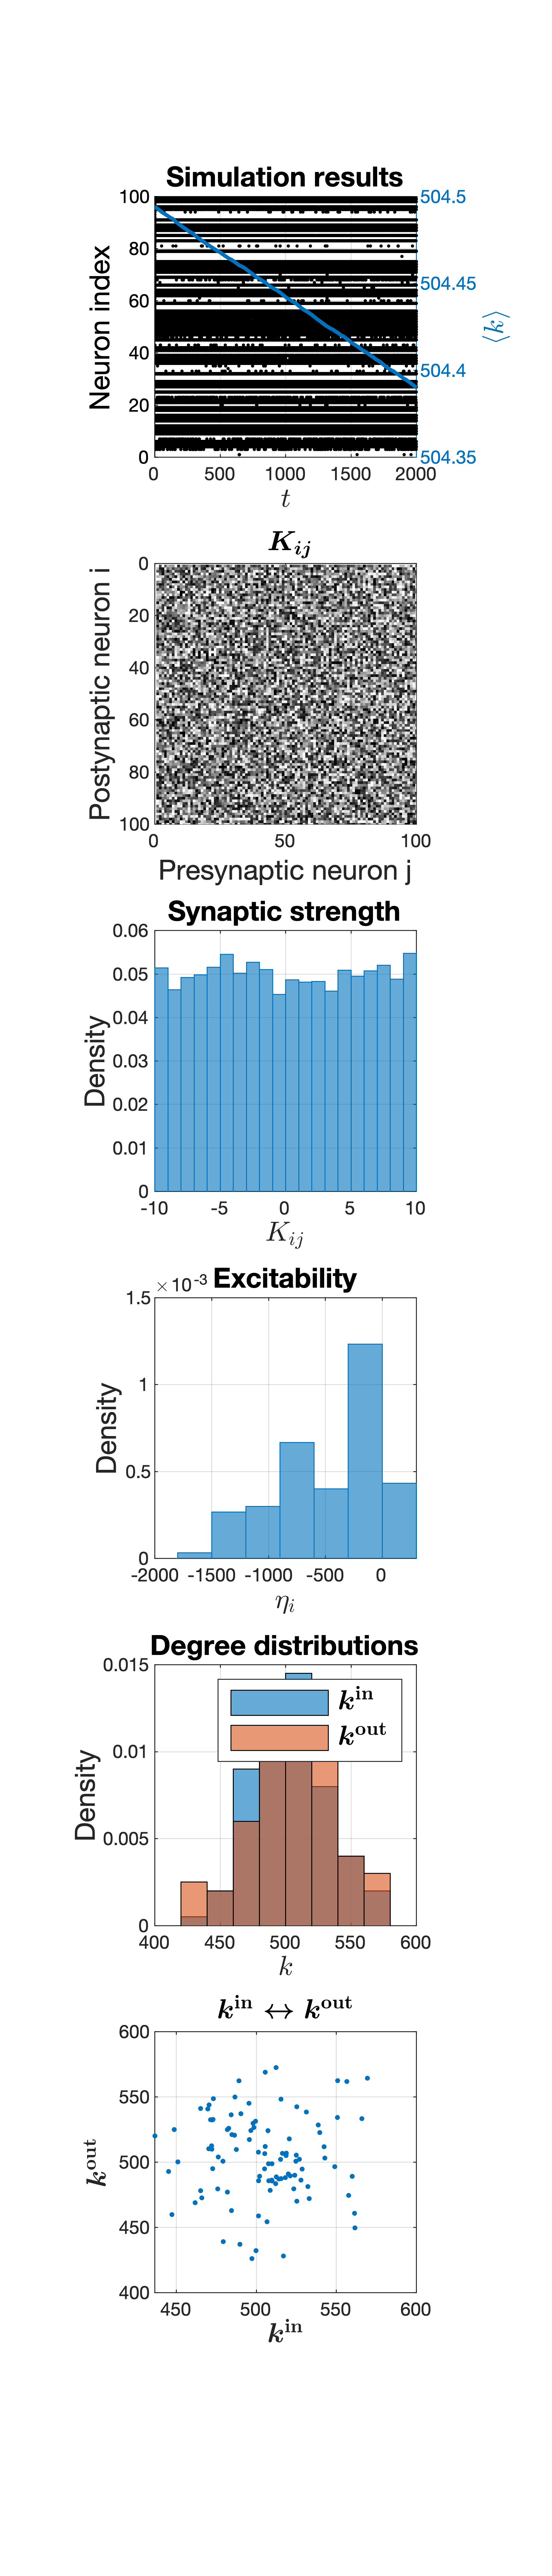
\includegraphics[width=\linewidth, trim={0 0 0 0 },clip]{../Figures/Learning/STDPandIPKempter.png}
   \caption{The window $W_K$.}
   \label{fig:STDPWK} 
\end{subfigure} \hfill
\begin{subfigure}[b]{0.32\linewidth}
   \centering
  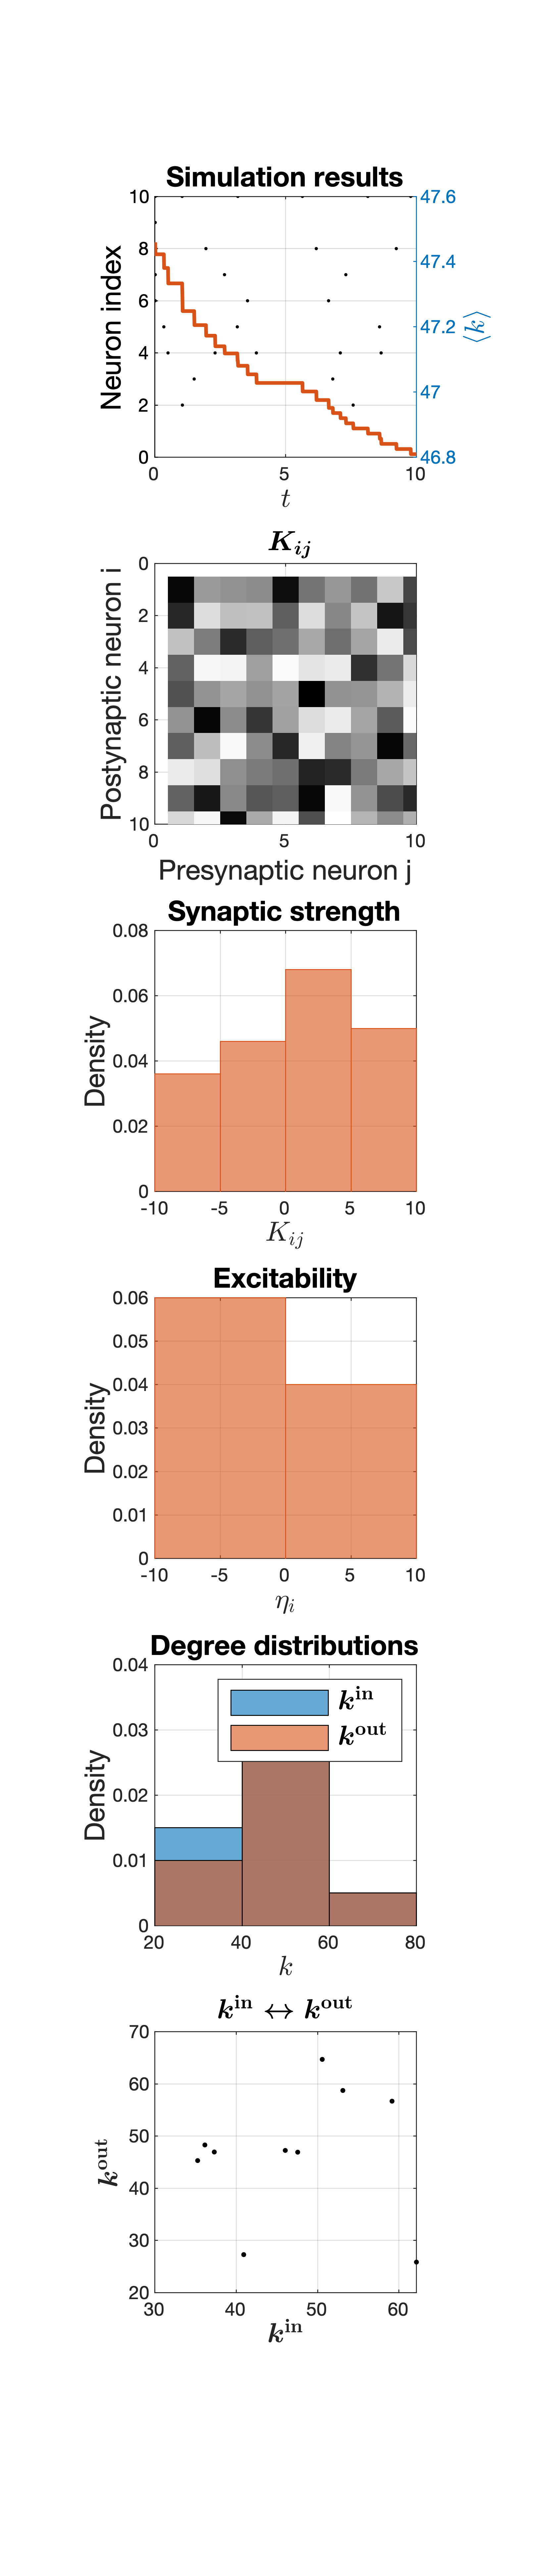
\includegraphics[width=\linewidth, trim={0 0 0 0},clip]{../Figures/Learning/STDPandIPSong.png}
   \caption{The window $W_S$.}
   \label{fig:STDPWS}
\end{subfigure} \hfill
\begin{subfigure}[b]{0.32\linewidth}
   \centering
  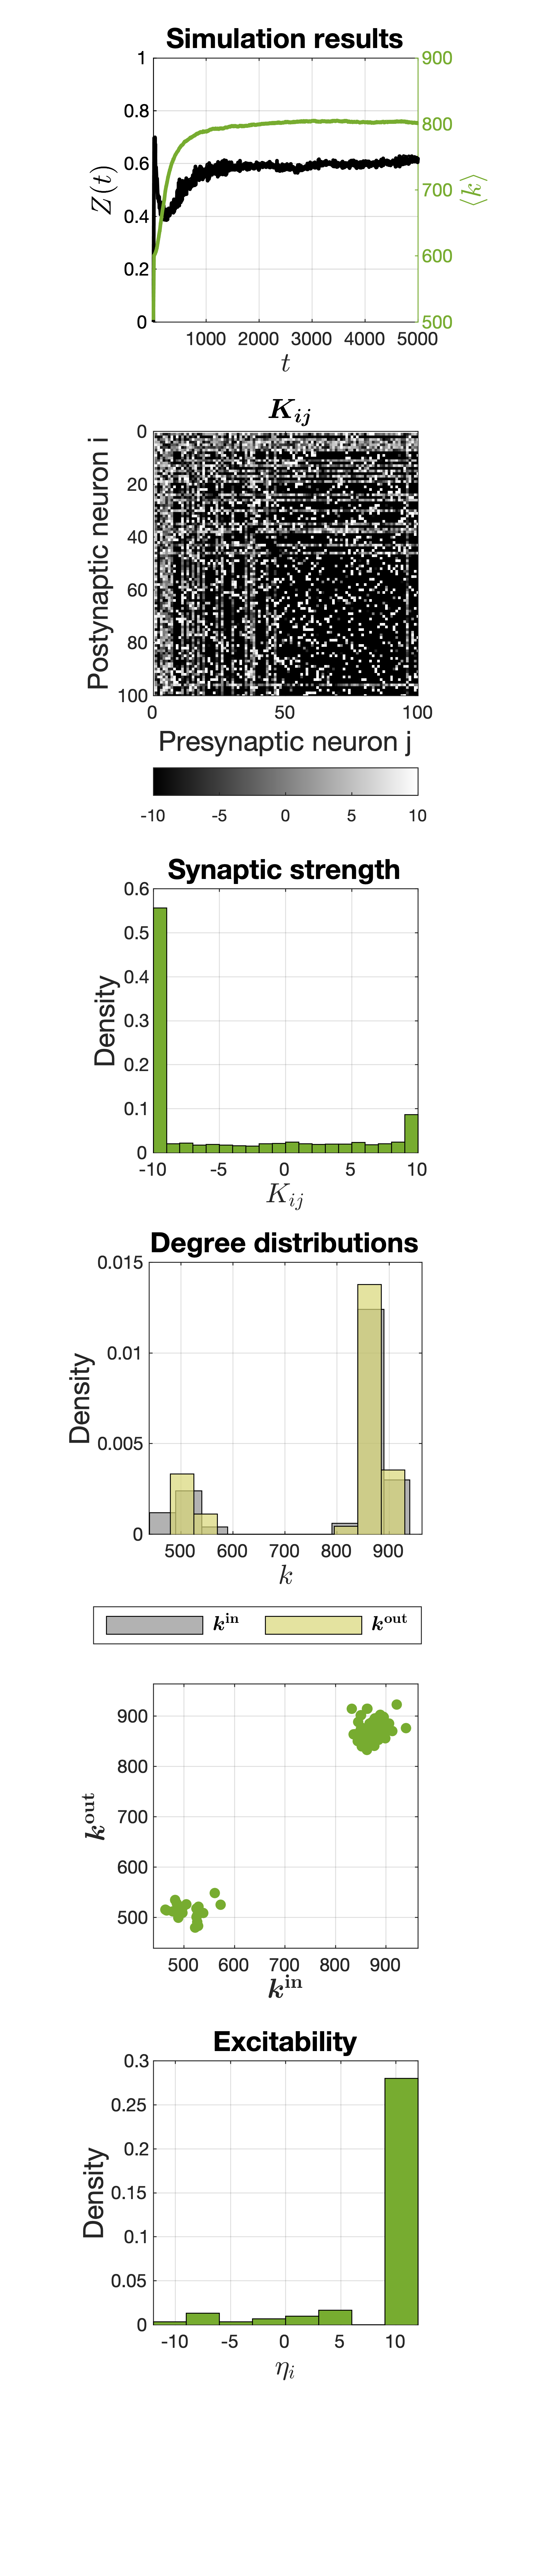
\includegraphics[width=\linewidth, trim={0 0 0 0},clip]{../Figures/Learning/STDPandIPChrolCannon.png}
   \caption{The window $W_C$.}
   \label{fig:STDPWC}
\end{subfigure}
   \caption{Results of the \STDP learning.}
   \label{fig:STDPresults}
\end{figure}



\subsection{Results}
\textcolor{red}{TODO}: \textsl{describe the emergent behaviour.}


% !TEX root = ../main.tex
\newpage
\section{Conclusion and Discussion} \label{sec:ConclusionAndDiscussion}
Starting from the Theta neuron model, we have holistically discussed its use in directed networks and described synchronisation of different network topologies, simplifying the analysis with the \MFR. We have proven that from random initial topological conditions, a regular network structure can appear. Obtaining these results is the first step towards a unification in the theory of the dynamics \textsl{on} and \textsl{of} networks. \\

Even though both fields have been well-established, currently there exists no theory that takes both approaches into account. The science of the different fields is scattered, a schism that is represented by the structure of this report. The only constant is the description of the behaviour of networks, which was rigorously adapted for this work. Going forward, it would be interesting to see whether a similar approach as in the \MFR can be taken: if the network dynamics can be represented per node degree, then why not find a learning strategy that allows for a coupling matrix defined on $\mathbb{N}^{N \times N}$? Or can we perhaps bin the node degrees so that even less equations are necessary for the \MFR to function? \\

These questions are the seed for a future investigation.

\subsection{Computational challenges of neuronal modelling and the \MFR}
Writing the software for simulating large networks of neurons and the \MFR was the biggest challenge in this work. A trade-off had to be made between speed and accuracy: testing a hypothesis is difficult when the simulation takes a long time. Therefore, the subject of the first exploration phase was all about which software to use. Extensions to Python written in \texttt{c} were found to run incredibly fast, though the framework for documentation of Matlab was eventually preferred for its
All code for this work is available on \href{https://github.com/simonaertssen/AdaptiveNeuronalNetworks}{GitHub} to promote future research.


\subsection{Further investigation of initial and final conditions}
The initial conditions of the different systems obtained in Chapter \ref{sec:initialconditions} by numerically solving for $f(z) = \| Z(0) - \bar{Z}(0) \|$ are satisfactory, but can be improved upon. The distribution of degrees over the attractive manifold can be taken into account by further analysis on the final conditions, and we should obtain a better understanding of the location of the manifold with respect to the resulting point in $\bar{Z}$. Then, a second condition can be added so that the numerical solution of $f$ converges to the manifold. 

In the current implementation, there is no objective function for the optimisation. $f$ is solved as an equality constraint so that the solution is exact and not just a minimum, and the constraint $| z | \leq 1$ is solved as an inequality. This leaves the objective function free to take the manifold into account: a metric like the Kullback-Leibler divergence can be introduced to take the target distribution into account. 


\subsection{A learning strategy with desirable properties}
In Chapter \ref{sec:HebbianLearningAndSynapticPlasticity}, two different learning strategies were presented, and in Chapter \ref{sec:EmergingNetworkTopologies} their functionality was discussed. The feedback loops between $W$ and $\Delta K$ make it hard to find a formulation that would guarantee a stable network topology, without the artificial bounds on $K$. Another challenge is allowing inhibitive \textsl{and} excitatory coupling, which no other work has touched upon.

A constant in the formulation of a learning strategy is the in- and outgoing spike trains: 
\begin{align}
\Delta K_{ij} \sim \sum_{t_{j}^{f}, \: t_i^{n} \in \mathcal{T}} \hspace{-2mm} W (t_{j}^{f}-t_i^{n} )
\end{align}
We can then easily punish nodes with large degrees by postulating:
\begin{align}
\Delta K_{ij} \sim - (K_{ij}) \circ \rvert K_{ij} \rvert
\end{align}
The Hadamard product $\circ$ ensures that the sign of the coupling strength is preserved, so that the restraint to halt the continuous potentiation works symmetrically, inspired by Oja's rule\cite{ChrolCannon2014}. We might also direct nodes with a low degree towards zero, or stimulate them to grow. The options explored by the machine learning community can be an inspiration for future research.


\subsection{Symmetry of the learned degree distributions}
The degree distributions resulting from the learning procedure in Chapters \ref{sec:STDPlearning} and \ref{sec:STDPandIPlearning} should be investigated further, as it appears that $\kinb$ and $\koutb$ are variates from the same univariate distribution. The impact of using a bimodal degree distribution, which was the result of using $W_C$, is currently unknown.

Perhaps the differences we observed between the \MFR and the solutions of the whole network in Chapter \ref{sec:resArbNetw} can be explained by the fact that fixed-degree and random networks have a degree distribution with $\kmean$ as the axis of symmetry, which the scale-free distribution does not have. The latter showed large differences between the two approaches.


\subsection{Synchronisation and spiking rate}
In accordance with most of the work conducted on the \MFR, the order parameter was used to measure synchrony in the network. In the context of \STDP and \IP, a better metric could have been the mean firing rate, the average neural activity of a node in the past:
\begin{align}
\rho(t)=\frac{1}{N} \sum_{j=1}^{N} \sum_{n} \delta\left(t-t_{j}^{n}\right)
\end{align}
The mean firing rate is related to the order parameter through:
\begin{align}
\rho(t) = \frac{1}{\pi} \Re \left(\frac{1-Z(t)^c}{1+Z(t)^c}\right)
\end{align}
In \cite{Montbrio2015}, a firing rate \MFR for networks of the Theta model was proposed, yielding a different light on the firing dynamics. This metric could easily be introduced in the analysis of the \MFR in Chapter \ref{sec:MFRSUndirected} and the learning procedures in Chapter \ref{sec:EmergingNetworkTopologies}.






\newpage
\bibliographystyle{utphys}
\small{\bibliography{references}}

% !TEX root = ../main.tex

\newpage
\appendix
\section{Appendix} \label{sec:Appendix}

\subsection{Transformation to the QIF model} \label{app:TransformationToQIF}
We prove that the transformation \eqref{eq:QIFtransformation} holds from the \QIF model \eqref{eq:QIFmodel} to the Theta model \eqref{eq:thetaneuron}.
\begin{align*}
V &\equiv \tan \left( \frac{\theta}{2} \right) \quad \longrightarrow \quad
\frac{\mathop{d V}}{\mathop{d t}} = \frac{1}{2 \cos ^{2}\left(\frac{\theta}{2}\right)} \frac{d \theta}{ \mathop{d t}}
\end{align*}
Insert into $\frac{\mathop{d V}}{\mathop{d t}}= V^2 + I$:
\begin{align*}
\frac{\mathop{d \theta}}{\mathop{d t}} &= 2\left(\cos ^{2}\left(\frac{\theta}{2}\right) \cdot \tan ^{2}\left(\frac{\theta}{2}\right)+\cos ^{2}\left(\frac{\theta}{2}\right) \cdot I \right) = 2\left(\sin ^{2}\left(\frac{\theta}{2}\right)+\cos ^{2}\left(\frac{\theta}{2}\right) \cdot I \right)
\end{align*}
Using $\cos ^{2}\left(\frac{\theta}{2}\right) = \frac{1+\cos \left(\frac{\theta}{2}\right)}{2}$ and $\sin ^{2}\left(\frac{\theta}{2}\right)=\frac{1-\cos \left(\frac{\theta}{2}\right)}{2}$:
\begin{align*}
\dot{\theta} &=2\left(\frac{1-\cos \theta}{2}+\left(\frac{1+\cos \theta}{2}\right) \cdot I \right) =(1-\cos \theta)+(1+\cos \theta) \cdot I
\end{align*}
This proves that the transformation \eqref{eq:QIFtransformation} is correct.

 
\subsection{Solutions to the QIF model} \label{app:ThetaModelSolutions}
Depending on the value of $I$, we can distinguish multiple solutions  \cite{Perez2020}. In all cases we can integrate through the separation of variables. Solutions are bound to start at $V(t_0)$, right after a spike has occured at $t=t_0$. 

\subsubsection{Solving for \texorpdfstring{$I < 0$}{TEXT}}
%Change variables: $I = -\tilde{I}^2$. Separate variables as $\frac{\mathop{dv}}{v^2 - \tilde{I}^2} = \mathop{dt}$ and integrate from $t = 0$:
\begin{align*}
\int_{V(t_0)}^{V(t)} \frac{\mathop{dv}}{v^2 - \tilde{I}^2} &= \int_{V(t_0)}^{V(t)} \frac{\mathop{dv}}{(v+\tilde{I})(v-\tilde{I})} 
= \frac{1}{2 \tilde{I}} \int_{V(t_0)}^{V(t)} \frac{\mathop{dv}}{v-\tilde{I}}-\frac{1}{2 \tilde{I}} \int_{V(t_0)}^{V(t)} \frac{\mathop{dv}}{v+\tilde{I}} \\
%&= \frac{1}{2 \tilde{I}} \log (v-\tilde{I}) -\frac{1}{2 \tilde{I}} \log (v+\tilde{I})\Big \rvert_{V(t_0)}^{V(t)} 
&= \frac{1}{2 \tilde{I}} \log \left(1-\frac{2 \tilde{I}}{v+\tilde{I}}\right) \Big \rvert_{V(t_0)}^{V(t)} 
= \int_{t_0}^t \mathop{d\tau} = t - t_0 \\
V(t) &= \lim_{V(t_0) \rightarrow -\infty} \frac{2 \sqrt{-I}}{1 - \left(1-\frac{2 \sqrt{-I}}{V(t_0)+\sqrt{-I}}\right)\cdot e^{2 (t - t_0)\sqrt{-I}}}-\sqrt{-I}\\
&= \frac{2 \sqrt{-I}}{1 - e^{2 (t - t_0) \sqrt{-I}}}-\sqrt{-I}
\end{align*}

\subsubsection{Solving for \texorpdfstring{$I = 0$}{TEXT}}
\begin{align*}
\int_{V(t_0)}^{V(t)} \frac{\mathop{dv}}{v^2} &= \frac{1}{v}\Big\rvert_{V(t_0)}^{V(t)} = - \frac{1}{V(t)} + \frac{1}{V(t_0)} = \int_{t_0}^t \mathop{d\tau} = t -t_0 \\
V(t) &= \lim_{V(t_0) \rightarrow - \infty} \frac{V(t_0)}{1-V(t_0)(t - t_0)} \underset{\frac{\infty}{\infty}}{\overset{\mathrm{H}}{=}} \frac{-1}{t - t_0}
\end{align*}

\subsubsection{Solving for \texorpdfstring{$I > 0$}{TEXT}}
%Separate the variables as $\frac{\mathop{dv}}{v^2 + I} = \mathop{dt}$ and integrate from $t=0$:
\begin{align*}
\int_{V(t_0)}^{V(t)} \frac{\mathop{dv}}{v^2 + I} &= \int_{V(t_0)}^{V(t)} \frac{I}{\left(\frac{v}{\sqrt{I}}\right)^2 + 1} \mathop{dv} 
\overset{x = \frac{v}{\sqrt{I}}}{\underset{\mathop{dx} = \frac{dv}{\sqrt{I}}}{=}} 
%\quad \longrightarrow \quad x = \frac{v}{\sqrt{I}} \quad \mathop{dx} = \frac{\mathop{dv}}{\sqrt{I}} \\
\int_{\frac{V(t_0)}{\sqrt{I}}}^{\frac{V(t)}{\sqrt{I}}} \frac{I}{x^2 + 1} \mathop{dx}= \frac{1}{\sqrt{I}} \arctan(x) \Big \rvert_{\frac{V(t_0)}{\sqrt{I}}}^{\frac{V(t)}{\sqrt{I}}} \\
&= \frac{1}{\sqrt{I}} \left( \arctan \left( \frac{V(t)}{\sqrt{I}} \right) - \arctan \left( \frac{V(t_0)}{\sqrt{I}} \right) \right) = 
\int_{t_0}^t \mathop{d\tau} = t - t_0 \\
V(t) &= \lim_{V(t_0) \rightarrow -\infty} \sqrt{I} \cdot \tan \left( (t - t_0) \sqrt{I} + \arctan \left( \frac{V(t_0)}{\sqrt{I}} \right) \right) = \sqrt{I} \cdot \tan \left( (t - t_0) \sqrt{I} - \frac{\pi}{2} \right) \\
&=  \sqrt{I} \cdot \cot \left( (t - t_0) \sqrt{I} \right) 
\end{align*}


\subsection{Frequency response of the neuron models} \label{app:ThetaModelFrequencyResponse}
The integral is solved like before, but now with the conditions of the spike:
\begin{align*}
T &= \lim_{a \rightarrow \infty} \int_{-a}^{a} \frac{I}{\left(\frac{v}{\sqrt{I}}\right)^2 + 1} \mathop{dv} 
\overset{x = \frac{v}{\sqrt{I}}}{\underset{\mathop{dx} = \frac{dv}{\sqrt{I}}}{=}} 
\lim_{a \rightarrow \infty} \int_{\frac{-a}{\sqrt{I}}}^{\frac{a}{\sqrt{I}}} \frac{I}{x^2 + 1} \mathop{dx}
= \lim_{a \rightarrow \infty} \frac{1}{\sqrt{I}} \arctan(x) \Big \rvert_{\frac{-a}{\sqrt{I}}}^{\frac{a}{\sqrt{I}}} \\
&= \frac{1}{\sqrt{I}} \left( \frac{\pi}{2} - \left( - \frac{\pi}{2} \right) \right)
= \frac{\pi}{\sqrt{I}}
\end{align*}
So the frequency of oscillation is proportional to $\sqrt{I}$. 


\subsection{Newton-Raphson root iteration} \label{app:NewtonRaphson}
We define the equilibria $\boldsymbol{x^\ast} \in \R^n$ of a multivariate function $\boldsymbol{f}(\boldsymbol{x}) : \R^n \rightarrow \R^n$ with $\boldsymbol{f}(\boldsymbol{x}) = \boldsymbol{0}$. Expanding $\boldsymbol{f}$ as a Taylor series, we obtain:
\begin{align*}
f_i(\boldsymbol{x} + \delta \boldsymbol{x}) =f_{i}(\boldsymbol{x}) + \sum_{j=1}^{n} \frac{\partial f_{i}(\boldsymbol{x})}{\partial x_{j}} \delta x_{j}+O\left(\delta \boldsymbol{x}^{2}\right) \approx f_{i}(\boldsymbol{x})+\sum_{j=1}^{n} \frac{\partial f_{i}(\boldsymbol{x})}{\partial x_{j}} \delta x_{j}, \qquad (i=1, \cdots, n)
\end{align*}
We can also write this in vector notation, by setting $\boldsymbol{J}(\boldsymbol{x}) = \nabla \boldsymbol{f}(\boldsymbol{x}) = \frac{d}{d\boldsymbol{x}} \boldsymbol{f}(\boldsymbol{x}) \in \R^{n \times n}$ 
\begin{align*}
\boldsymbol{f}(\boldsymbol{x}+\delta \boldsymbol{x}) &\approx\left[\begin{array}{c}f_{1}(\boldsymbol{x}) \\ \vdots \\ f_{N}(\boldsymbol{x})\end{array}\right] 
+ \left[\begin{array}{ccc}\frac{\partial f_{1}}{\partial x_{1}} & \cdots & \frac{\partial f_{1}}{\partial x_{N}} \\ \vdots & \ddots & \vdots \\ \frac{\partial f_{N}}{\partial x_{1}} & \cdots & \frac{\partial f_{N}}{\partial x_{N}}\end{array}\right]
\left[\begin{array}{c}\delta x_{1} \\ \vdots \\ \delta x_{N}\end{array}\right] 
=\boldsymbol{f}(\boldsymbol{x})+\boldsymbol{J}(\boldsymbol{x}) \delta \boldsymbol{x} 
\end{align*}
By assuming $\boldsymbol{f}(\boldsymbol{x}+\delta \boldsymbol{x}) = 0$ we can find that $\delta \boldsymbol{x} = -\boldsymbol{J}^{-1}( \boldsymbol{x}) \boldsymbol{f}(\boldsymbol{x})$ so that $\boldsymbol{x} + \delta \boldsymbol{x} =  \boldsymbol{x} - \boldsymbol{J}^{-1} (\boldsymbol{x}) \boldsymbol{f}(\boldsymbol{x})$. This expression converges to $\boldsymbol{x^\ast}$. When the equations are nonlinear, the equations converge to the real root as $\boldsymbol{x}_k =  \boldsymbol{x}_k - \boldsymbol{J}^{-1} ( \boldsymbol{x}_k)\boldsymbol{f}(\boldsymbol{x}_k)$.


\subsection{Jacobian of the Ott-Antonsen manifold}
Starting from \eqref{eq:OttAntonsenSystemFull}, we separate the real and imaginary parts of $z(\k, t)$ in $x_{\k} = x(\k, t)$ and $y_{\k} = y(\k, t)$:
\begin{align*}
\frac{\partial z_{\k}}{\partial t} &= -\frac{\ic}{2} \cdot \left( x_{\k}^2 + \ic 2x_{\k}y_{\k} - y_{\k}^2 - 2x_{\k} - \ic 2y_{\k} +1\right) + \frac{1}{2} \cdot \left( x_{\k}^2 + \ic 2x_{\k}y_{\k} - y_{\k}^2 + 2x_{\k} + \ic 2y_{\k} +1 \right) \cdot I_{\k}\\
I_{\k} &= -\sigma_{\k} + \ic \eta_{0, \k} + \ic H_{2_{\k}} \\
H_{2_{\k}} &= \frac{\kappa}{\kmean} \sum_{\kacc \in \K} P\left(\kacc\right) \: a\left(\kacc \rightarrow \k\right) \cdot \left( 1 + \frac{x_{\k}^2}{3} - \frac{4}{3} x_{\k} \right)
\end{align*}
Taking the dynamics per real and imaginary value yields:
\begin{align*}
\frac{\partial x_{\k}}{\partial t}
&=f_{\k} \left(x_{\k}, y_{\k} \right) \\ 
&=(x_{\k}-1) y_{\k}-\frac{(x_{\k}+1)^{2}-y_{\k}^{2}}{2} \sigma_{\k} + (x_{\k}+1) y_{\k} \left[\eta_{0}+ H_{2_{\k}}\right] \\ 
\frac{\partial x_{\k}}{\partial t}
&= g_{\k} \left(y_{\k}, y_{\k} \right) \\ 
&=-\frac{(x_{\k}-1)^{2}-y_{\k}^{2}}{2}-(x_{\k}+1) y_{\k} \sigma_{\k} + \frac{(x_{\k}+1)^{2}-y_{\k}^{2}}{2} \cdot \left[\eta_{0} + H_{2_{\k}} \right] 
\end{align*}
And the Jacobian is found from the partial derivatives of $f$ and $g$:
\begin{align*}
\frac{\partial f_{\k}}{\partial x_{\k}} &= y_{\k}-(x_{\k}+1) \sigma_{\k}-y_{\k} \left[\eta_{0} + \kappa \cdot H_{2_{\k}} \right] + (x_{\k}+1) y_{\k} \frac{\partial H_{2_{\k}}}{\partial x_{\k}}\\
\frac{\partial f_{\k}}{\partial y_{\k}} &= (x_{\k}-1)+y_{\k} \sigma_{\k} + (x_{\k}+1) \left[\eta_{0} + H_{2_{\k}} \right] \\
\frac{\partial g_{\k}}{\partial x_{\k}} &= -(x_{\k} - 1) - y_{\k}  \sigma_{\k} + (x_{\k} + 1) \left[\eta_{0} + H_{2_{\k}} \right] + \left( \frac{(x_{\k} + 1)^2 - y_{\k}^2}{2} \right) \frac{\partial H_{2_{\k}}}{\partial x_{\k}} \\
\frac{\partial g_{\k}}{\partial y_{\k}} &= y_{\k} - (x_{\k} + 1) \sigma_{\k} - y_{\k} \left[\eta_{0} + H_{2_{\k}} \right] \\
\frac{\partial H_{2_{\k}}}{\partial x_{\k}} &= \frac{\kappa}{\langle k\rangle} P\left(\k\right) \: a\left(\k \rightarrow \k\right) (x_{\k}-2) \frac{2}{3} \\
\frac{\partial H_{2_{\k}}}{\partial y_{\k}} &= 0 
\end{align*}

And the off-diagonal elements, the nodes represented by degree $\kacc$:
\begin{align*}
\frac{\partial f_{\k}}{\partial x_{\kacc}} &= (x_{\k}+1) y_{\k} \frac{\partial H_{2_{\k}}}{\partial x_{\kacc}}\\
\frac{\partial f_{\k}}{\partial y_{\kacc}} &= 0 \\
\frac{\partial g_{\k}}{\partial x_{\kacc}} &= \left( \frac{(x_{\k} + 1)^2 - y_{\k}^2}{2} \right) \frac{\partial H_{2_{\k}}}{\partial x_{\kacc}} \\
\frac{\partial g_{\k}}{\partial y_{\kacc}} &= 0\\
\frac{\partial H_{2_{\k}}}{\partial x_{\kacc}} &= \frac{\kappa}{\langle k\rangle} P\left(\kacc\right) \: a\left(\kacc \rightarrow \k\right)(x_{\kacc}-2) \frac{2}{3} \\
\frac{\partial H_{2_{\k}}}{\partial y_{\kacc}} &= 0
\end{align*}


\label{LastPage}~







\end{document}
